\documentclass[hidelinks,a4paper,12pt]{report}

\usepackage[utf8x]{inputenc}
\usepackage[T2A]{fontenc} 
\usepackage[serbianc]{babel}
\usepackage[colorlinks = true,urlcolor = blue]{hyperref}
\usepackage{setspace, amsmath, amsfonts, amssymb, amsthm, enumerate, graphicx, color}
\usepackage[left=1in, right=1.0in, top=1.0in, bottom=1.0in]{geometry}
\usepackage{listings}
\usepackage{algorithm}
\usepackage{algpseudocode}
\usepackage{booktabs}
\usepackage{siunitx}

\newcommand{\HRule}{\rule{\linewidth}{0.5mm}}
\newcommand{\conj}{\overline}
\newcommand{\trig}{r(\cos\varphi+i\sin\varphi)}	
\newcommand{\trign}{r^n(\cos(n\varphi)+i\sin(n\varphi))}
\newcommand{\trigj}{r(\cos\alpha+i\sin\alpha)}
\renewcommand{\vec}{\overrightarrow}

%% Custom colours
\definecolor{darkgreen}{rgb}{0.0, 0.42, 0.24}
\definecolor{light-gray}{gray}{0.85}
% C++ Code%00
\definecolor{mygreen}{rgb}{0,0.6,0}
\definecolor{mygray}{rgb}{0.5,0.5,0.5}
\definecolor{mymauve}{rgb}{0.58,0,0.82}

\lstset{ %
  backgroundcolor=\color{white},   % choose the background color; you must add \usepackage{color} or \usepackage{xcolor}
  basicstyle=\footnotesize\ttfamily,        % the size of the fonts that are used for the code
  %belowskip=-0.8\baselineskip,
  breakatwhitespace=false,         % sets if automatic breaks should only happen at whitespace
  breaklines=true,                 % sets automatic line breaking
  captionpos=b,                    % sets the caption-position to bottom
  commentstyle=\color{mygreen},    % comment style
  deletekeywords={...},            % if you want to delete keywords from the given language
  escapeinside={\%*}{*)},          % if you want to add LaTeX within your code
  extendedchars=true,              % lets you use non-ASCII characters; for 8-bits encodings only, does not work with UTF-8
  frame=false,                    % adds a frame around the code
  keepspaces=true,                 % keeps spaces in text, useful for keeping indentation of code (possibly needs columns=flexible)
  keywordstyle=\color{blue},       % keyword style
  language=C++,                 % the language of the code
  literate={~} {\mytilde}{1},
  morekeywords={*,...},            % if you want to add more keywords to the set1
  numbers=left,                    % where to put the line-numbers; possible values are (none, left, right)
  numbersep=5pt,                   % how far the line-numbers are from the code
  numberstyle=\tiny\color{mygray}, % the style that is used for the line-numbers
  rulecolor=\color{black},         % if not set, the frame-color may be changed on line-breaks within not-black text (e.g. comments (green here))
  showspaces=false,                % show spaces everywhere adding particular underscores; it overrides 'showstringspaces'
  showstringspaces=false,          % underline spaces within strings only
  showtabs=false,                  % show tabs within strings adding particular underscores
  stepnumber=1,                    % the step between two line-numbers. If it's 1, each line will be numbered
  stringstyle=\color{mymauve},     % string literal style
  tabsize=2,                       % sets default tabsize to 2 spaces
  title=\lstname                   % show the filename of files included with \lstinputlisting; also try caption instead of title
}


\raggedbottom                           % try to avoid widows and orphans
\sloppy
\clubpenalty1000%q
\widowpenalty1000%

\renewcommand{\baselinestretch}{1.1}    % adjust line spacing to make
                                        % more readable


\begin{document}

\bibliographystyle{plain}



\begin{titlepage}

\begin{center}


% Upper part of the page   

\textsc{\Huge \textbf{Универзитет у Београду}} \\[1cm]
\textsc{\Huge \textbf{Електротехнички факултет}}\\[5cm]

\textsc{\Huge \textbf{Дипломски рад }}\\[0.5cm]
\textsc{\large{\textbf{из програмирања мобилних уређаја}}}
\\[4cm]

% Title
\HRule \\[0.8cm]
{ \Huge \bfseries Android апликација - Игра балансирања лоптице}\\[0.4cm]

\HRule \\[4cm]

% Author and supervisor
\begin{minipage}{0.55\textwidth}
\begin{flushleft} \large
\emph{Аутор}\\
Ђорђе Живановић, 0033/2013\\
\end{flushleft}
\end{minipage}
\begin{minipage}{0.4\textwidth}
\begin{flushright} \large
\emph{Ментор} \\
Др Саша Стојановић
\end{flushright}
\end{minipage}



\vfill

% Bottom of the page
{\large Београд, \today}

\end{center}

\end{titlepage}

\tableofcontents

\renewcommand{\bibname}{Литература и линкови}
\pagenumbering{arabic}
\renewcommand{\chaptername}{ Глава}


\chapter{Увод}
\emph{Основни циљ пројекта био је да истражим Android API\footnote{Application programming interface} који се користи за прављење апликација за Android уређаје. Да бих у потпуности разумео његову употребу и организацију кода у апликацијама за Android, морао сам да приступим изазову прављења игрице попут ове. Поред Android API-а први пут сам се сусрео са проблемима моделирања физике у рачунарској графици. У овом поглављу сам се осврнуо на мотивацију за имплементацију на овај начин, као и изазове са којима сам се сусрео у изради пројекта. }
\section{Мотивација}
Вештина коју програмер мора да има је прилагођавање новонасталим ситуацијама и решавање проблема који дођу у њима. 
\\ \indent Прављење великог пројекта са  непознатим API-ем један од великих изазова на које сам наишао. Први корак у томе био је предмет програмирање мобилних уређаја (\cite{PMU}), који сам слушао и на ком сам научио основне ствари које нуди Android API. Други корак је било злостављање AndroidDeveloper сајта (\cite{AndroidDeveloper})на ком смо налазили на предмету одговарајуће класе, методе, константе, чланке који су нам омогућавали прављење жељених апликација. Последњи корак на који се прибегавало кад проблем није могао бити решен је StackOverflow (\cite{StackOverflow}). Наведени кораци су ми омогућавали и давали мотивацију за даљи рад у борби са непознатим.
\\ \indent Други велики мотив био је рачунарска графика. Пошто као сваки мали дечак у великом телу сам имао жељу да научим како раде игрице попут GTA (\cite{GTA}). Први корак ка томе било је моделирање нечега што се може назвати модел судара. Дати пројекат је био изазован у погледу организације кода за модел судара, јер су сви делови уско спрегнути.
\\ \indent Последњи мотив, а можда и најважнији била је организација кода у великом пројекту као што је овај, која омогућава брзу проширивост и лагано додавање нових функционалнсти, мењање постојећих модела судара... Ово је врхунац знања сваког програмера.

\section{Постојећа решења}
Битна особина коју програмер мора да поседује је способност да чита туђи код и да прилагођава својој имплементацији. Књига која ми је је помогла да направим модел судара какав је у игрици је \cite{EngBook}. Она ми је омогућила да добијем увид у организацију кода и она је само била увод у моје решење. Поред тога модификовани су разни модели и тестирани за потребе. За доста реалнији модел постоји пуно више радова на интернету, али за почетну идеју користио сам упрошћену имплементацију једног модела из књиге \cite{EngBook}, која се налази у линку: 		\cite{ModCol}.

\section{Коришћени алати}
Користио сам прорамски језик Java искључиво јер омогућава лакшу израду пројекта и лакше дебаговање. У комбинацији са Java коришћeн је xml за израду GUI\footnote{Graphical User Interface}.Коришћен је Android Studio\footnote{\url{https://developer.android.com/studio/index.html}} који ми је дао лагодност у погледу дебаговања, build-овања и праћења промена. Он омогућава интегрисани рад са системима за праћење ревизија попут Git. У наставку се налази списак свих коришћених алата:
\begin{table}[H]\centering
\begin{tabular}{ l  l } \toprule
{\bf Алат} & {\bf Сврха}\\ \midrule
{\tt AndroidStudio 2.3.3} & IDE\\
{\tt compileSdkVersion 25.0.1} & систем за build-овање уграђен у AndroidStudio\\
{\tt SourceTree 2.1.2.5.} & Систем за ревизију\\
\TeX Maker 4.5 & \LaTeX\ уређивач\\
\bottomrule
\end{tabular}
\caption{Алати коришћени при развоју пројекта.} \label{UsedTools}
\end{table}


\section{Структура}
У глави  \ref{Collision} биће причано о моделу који судара који је коришћен и зашто су биране његове компоненте. У глави \ref{Graphics} биће описан систем за исцртавање екрана. У глави \ref{Architecture} биће описана софтверска архитектура (пројектни обрасци, организација кода). У глави \ref{UseCases} биће наведени неки случајеви коришћења система и како се систем понаша у одређеним тренуцима. У глави \ref{Conclusion} биће наведени закључци, да ли систем може да се побоља, да ли могу да се додају нове функционалности и сл.


	
\chapter{Резултати} \label{UseCases}

\section{Почетни екран} \label{UseCases:Main}

\begin{figure}[htb!]
\begin{center}
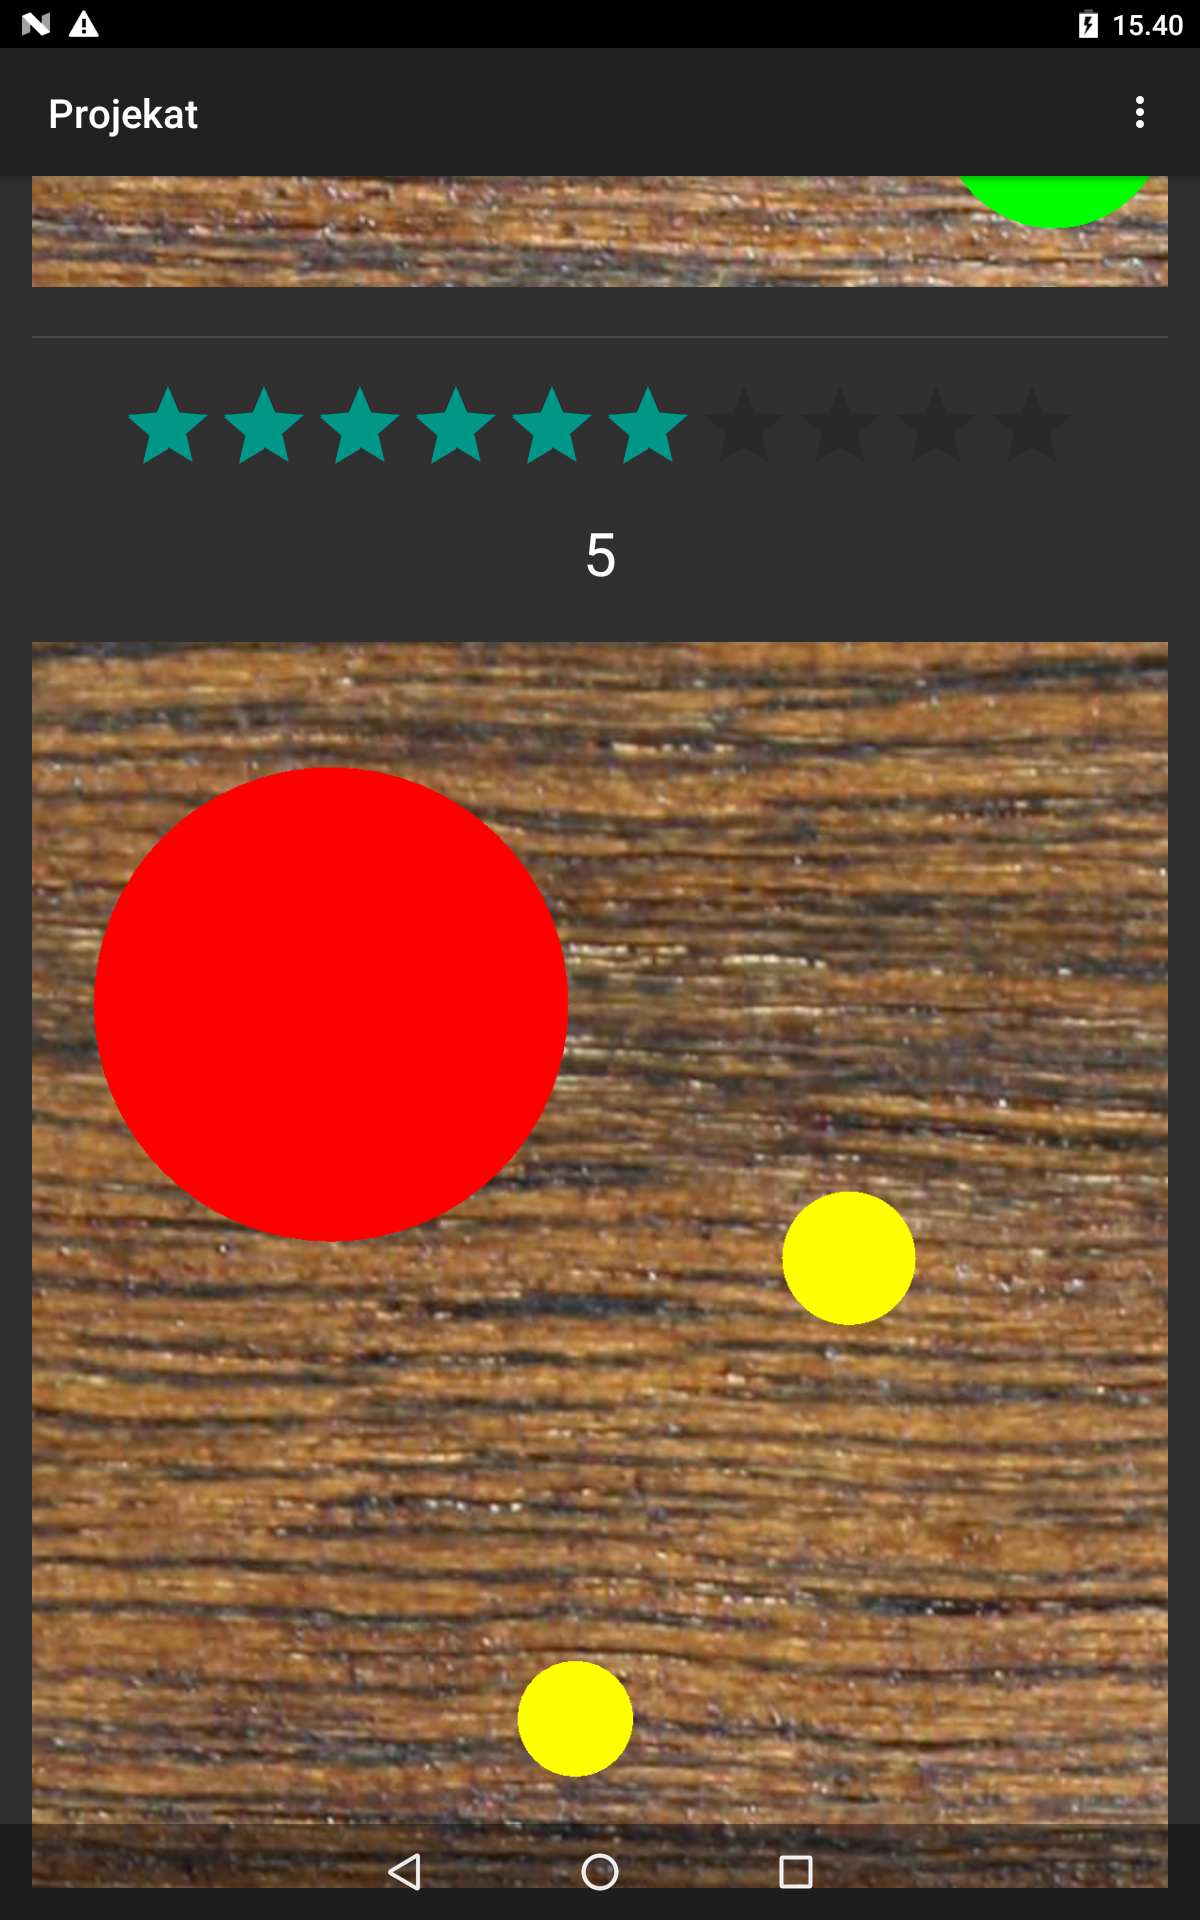
\includegraphics[scale=.1]{pictures/main/Basic}
\caption{Почетни екран}\label{fig:mainBasic}
\end{center}
\end{figure}
Кад корисник покрене апликацију појављује му се листа полигона које може да игра, са изгледом полигона (слика \ref{fig:mainBasic}). Такође изнад изгледа полигона налазе се његово име и тежина. Ово омогућава да кориснику почетнику одабере ниво прикладан за њега, или експерту да се окуша са нечим тежим. Изглед полигона је скалиран да одговара оном који ће бити у игрици. Кликом на било који од полигона у листи покреће му се игра за тај полигон.

\begin{figure}[htb!]
\begin{center}
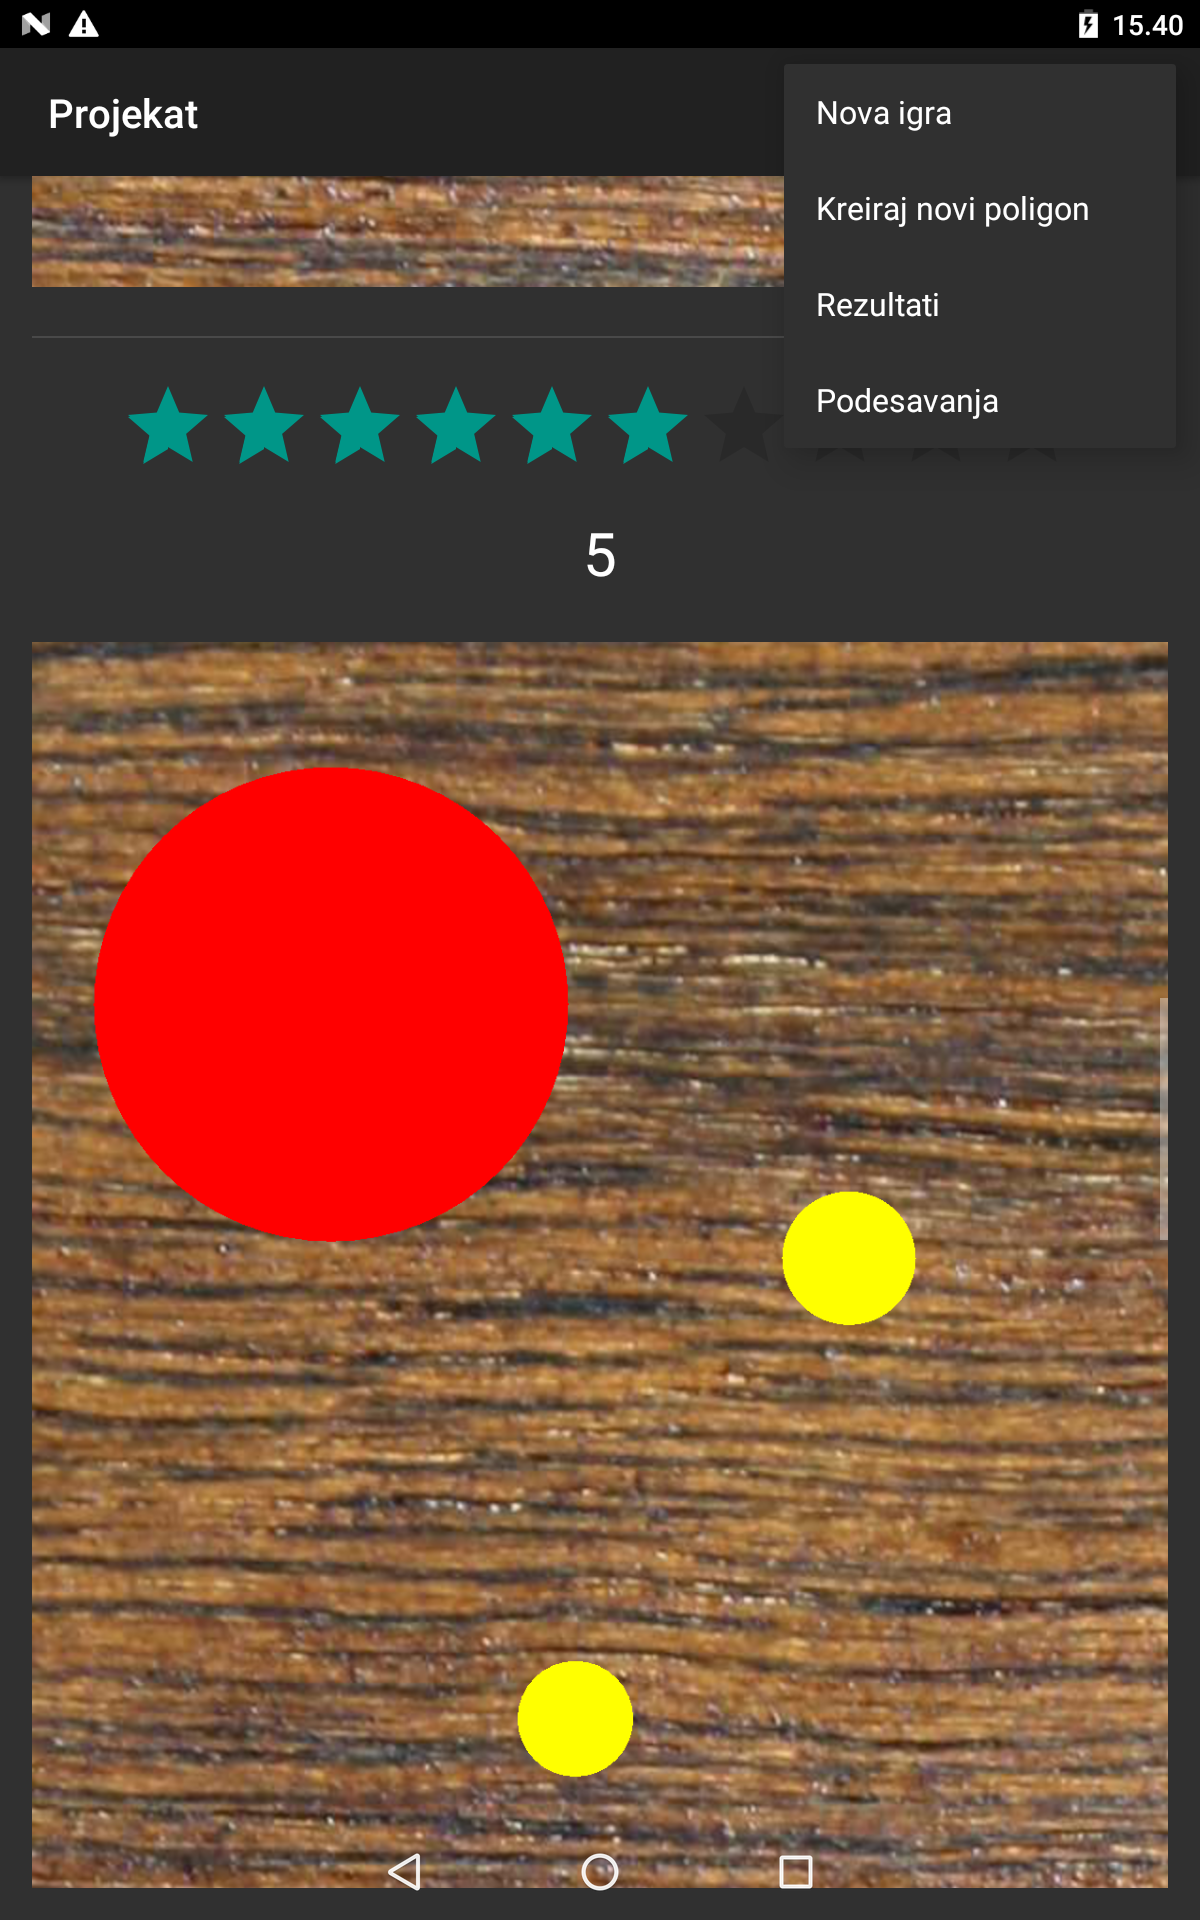
\includegraphics[scale=.1]{pictures/main/Menu}
\caption{Мени}\label{fig:mainMenu}
\end{center}
\end{figure}
Корисник све време на врху прозора има мени који отвара ако прстом кликне на три тачке. Из менија који се појави (слика \ref{fig:mainMenu}) корисник може да одабере једну од 4 опције. Прва опција започиње нову игру, али у режиму од више нивоа који су насумично генерисани. Друга опција отвара нови екран у ком корисник прави свој полигон. Трећа опција отвара нови екран резултати, где корисник може да види све резултате претходних игри, као и других играча. Четврта опција отвара подешавања за игру, која корисник може да мења.

\begin{figure}[htb!]
\begin{center}
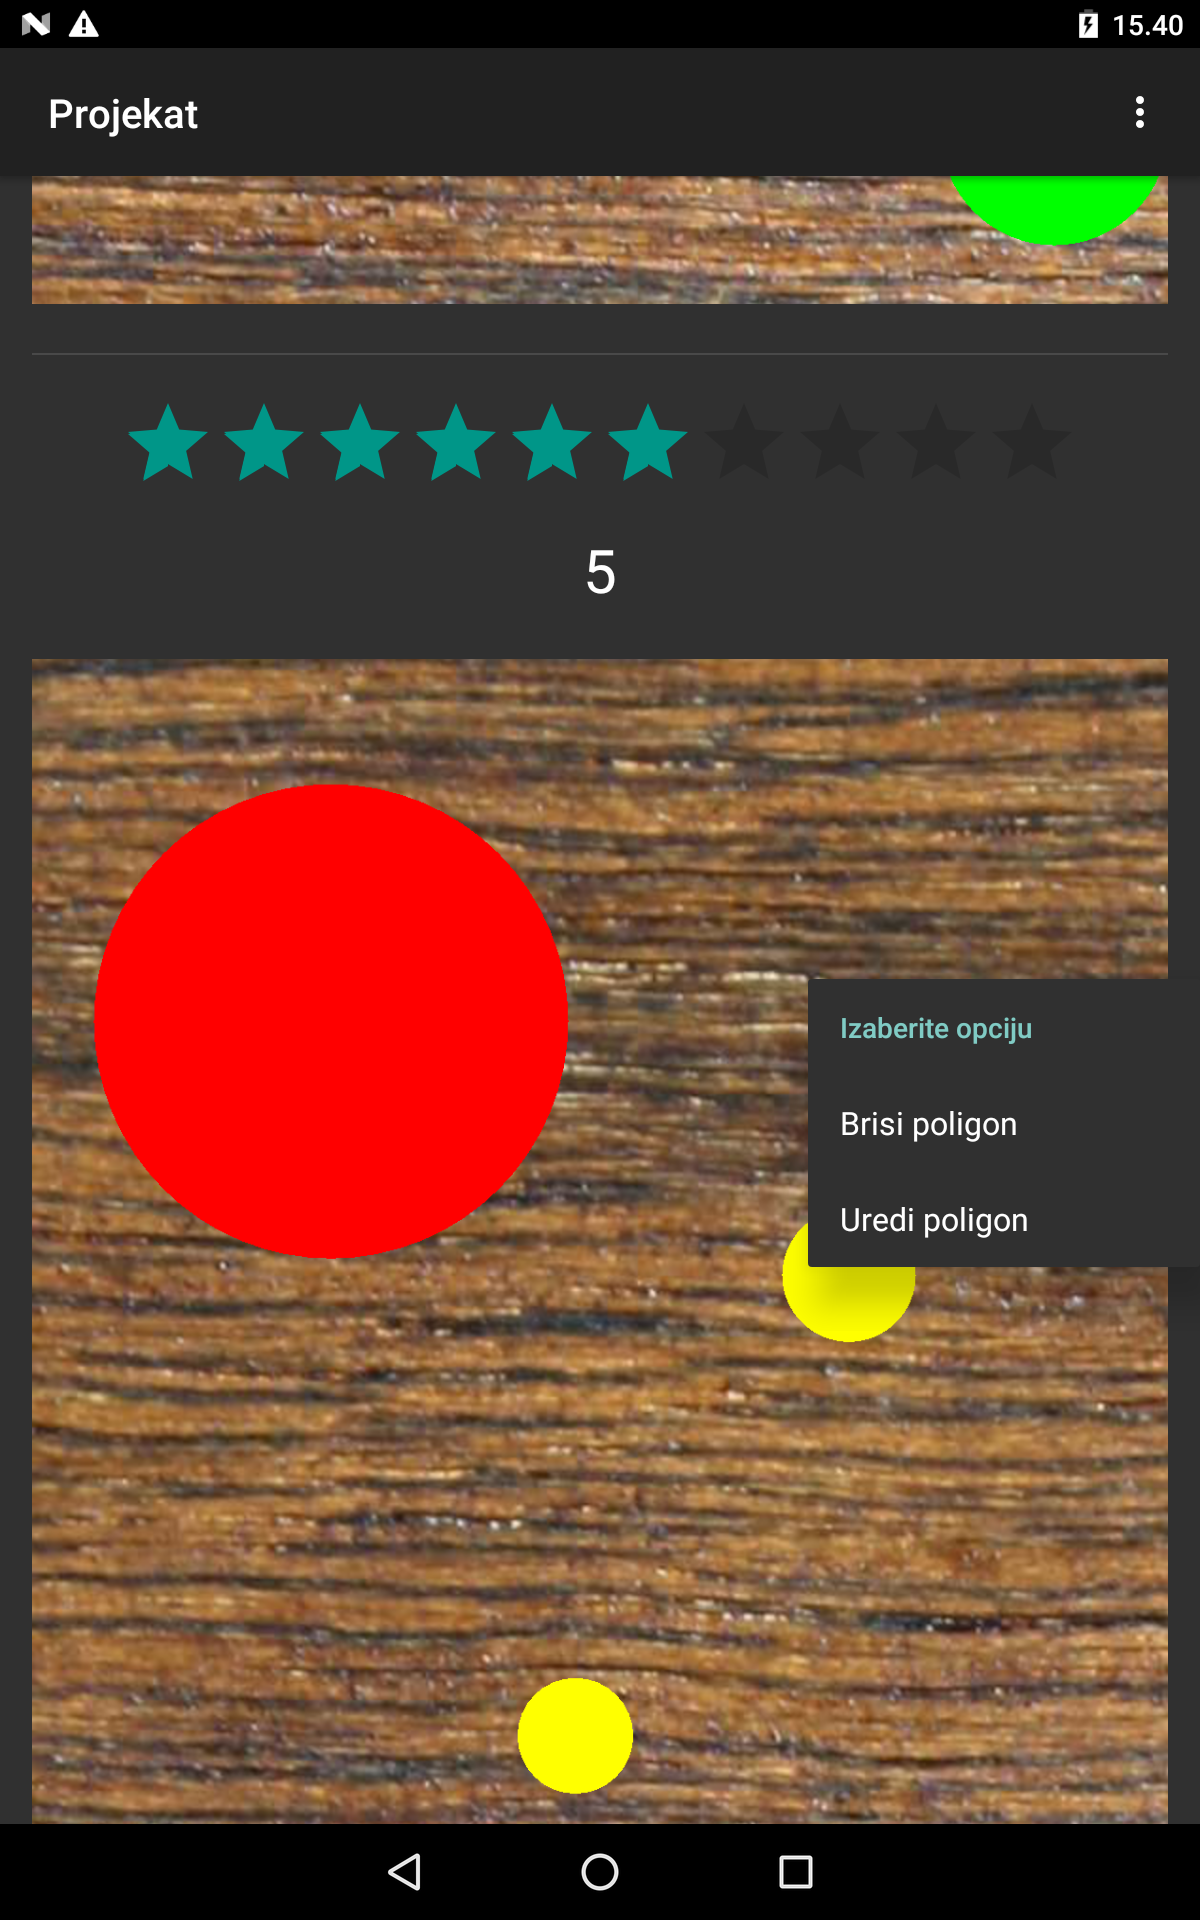
\includegraphics[scale=.1]{pictures/main/PolygonMenu}
\caption{Падајући мени везан за полигон}\label{fig:mainPolygonMenu}
\end{center}
\end{figure}
Корисник задржавањем прста на полигон добија падајући мени (слика \ref{fig:mainPolygonMenu}) са две опције. Прва опција брише полигон из целе игре. А друга омогућава његово уређивање, тако што отвара нови прозор са датим полигоном.

\section{Игра}\label{UseCases:Game}
\begin{figure}[htb!]
\begin{center}
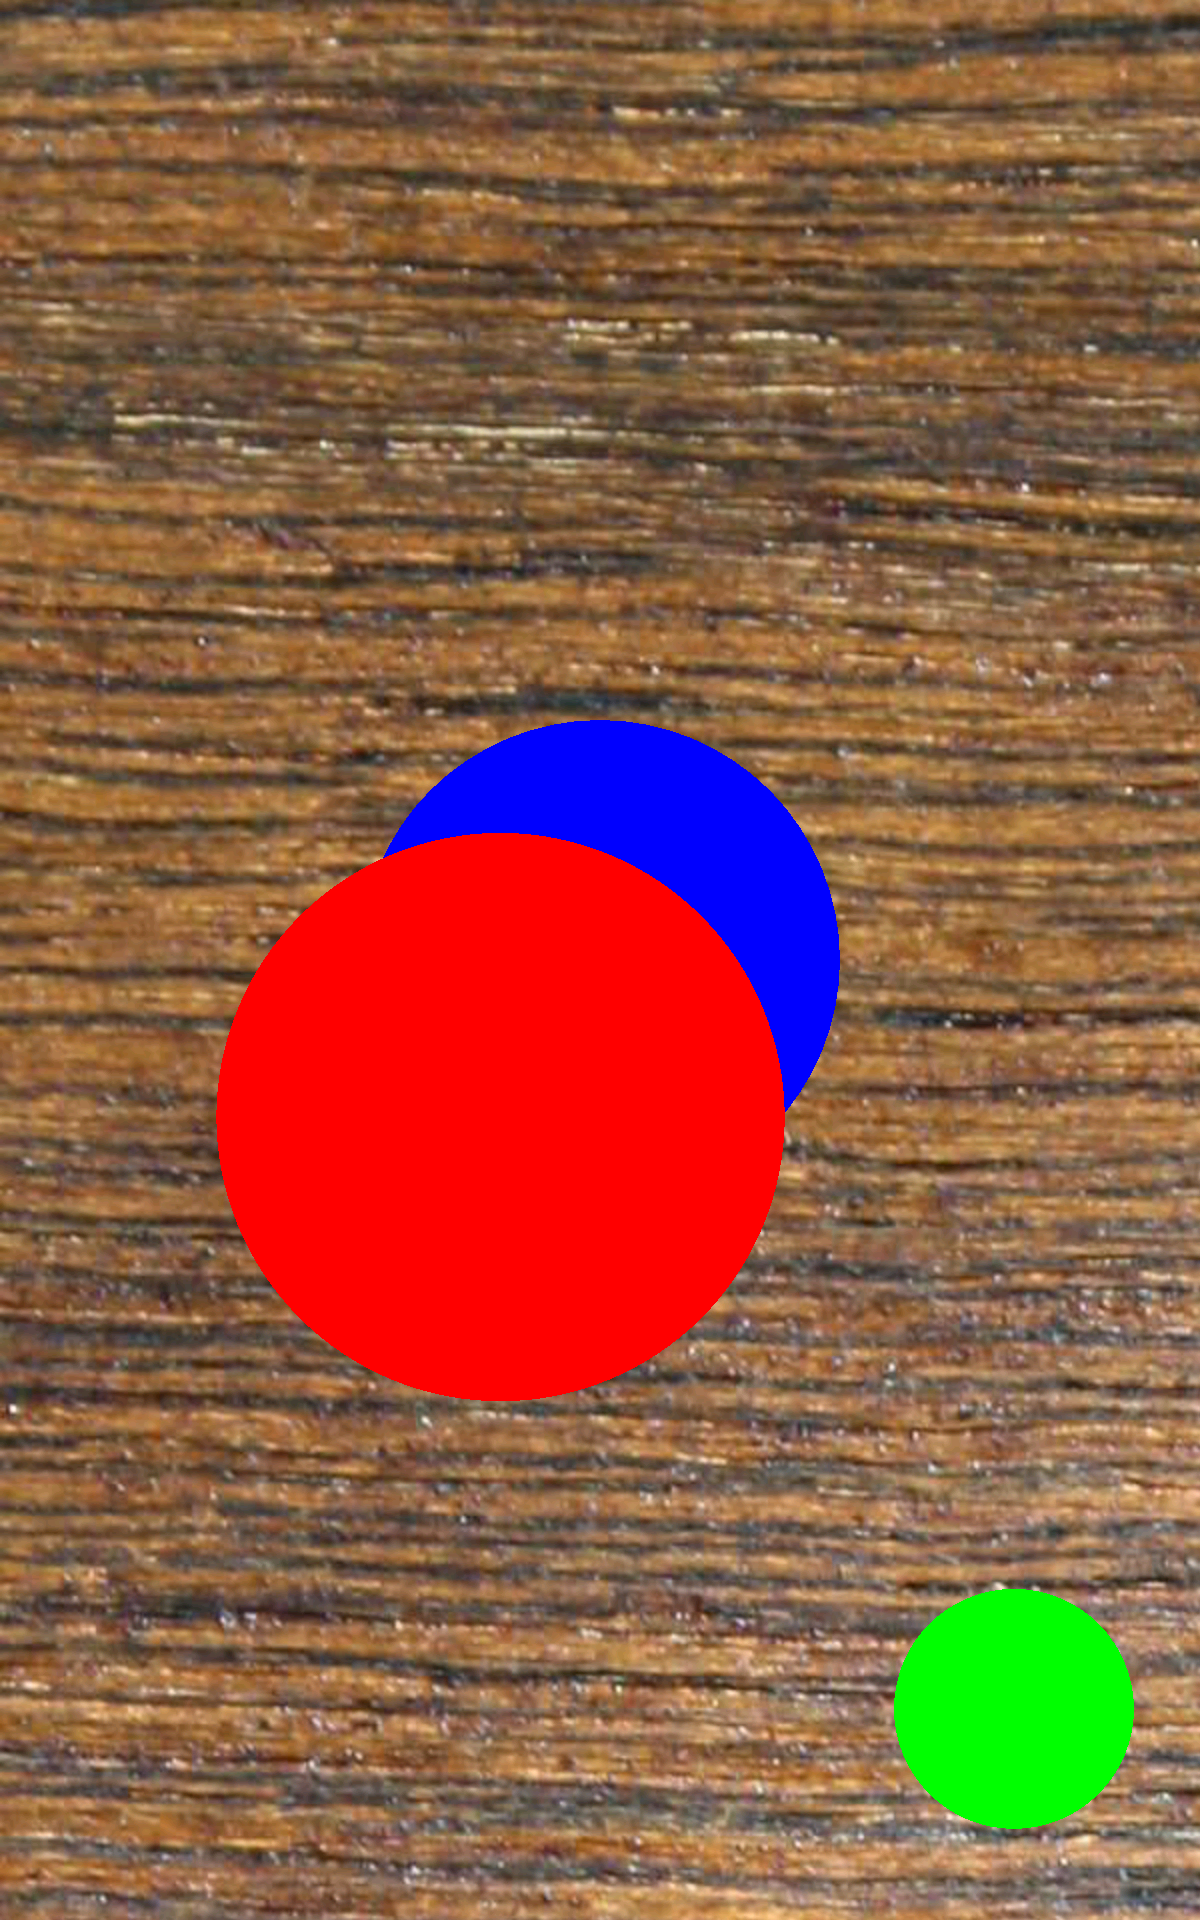
\includegraphics[scale=.1]{pictures/game/game}
\caption{Тренутак у игри}\label{fig:gameGame}
\end{center}
\end{figure}


Постоје два мода играња. Први мод је обичан у ком је циљ да црвену лопту корисник убаци у зелену рупу за што краће време (слика \ref{fig:gameGame}). Што му је време краће, биће боље рангиран на листи за тај полигон. Други мод је авантуристчки који омогућава кориснику да игра десет насумичних нивоа заредом који су поређани по растућој тежини и биће рангиран на посебној листи  за тај мод. Корисник има неколико типова препрека на које може да наиђе (слика \ref{fig:createPolygonBasic}). Типови препрека:
\begin{enumerate}
	\item Зид (ивица екрана и жути правоугаоник) - лопта се одбија од зида под истим углом којим улази. Губитак енергије током судара зависи од коефицијента подешеног у подешавањима.
	\item Стуб (жути круг) - исто као зид, са тим да је кружног облика.
	\item Амбис (црни круг) - лопта кад упадне у њега играч губи игру.
	\item Вртлог (плави круг) - покушава да увуче лопту у њега, и потом у зависности од брзине баца из њега или га врти.
	\item Крај (зелени круг) - кад лопта упадне у њега корисник је победио дати полигон.\footnote{Амбис, вртлог и крај кад лопта их дотакне вуку је ка себи одређеном силом}
\end{enumerate}
Лопта све време добија брзину у зависности од силе која делује на Android уређаја. На лопту у сваком тренутку делује трење од стране подлоге које покушава да је врати у стање мировања. У сваком тренутку корисник може да изађе из одговарајућег полигона, али неће му бити сачувано ништа што је играо.
\begin{figure}[htb!]
\begin{center}
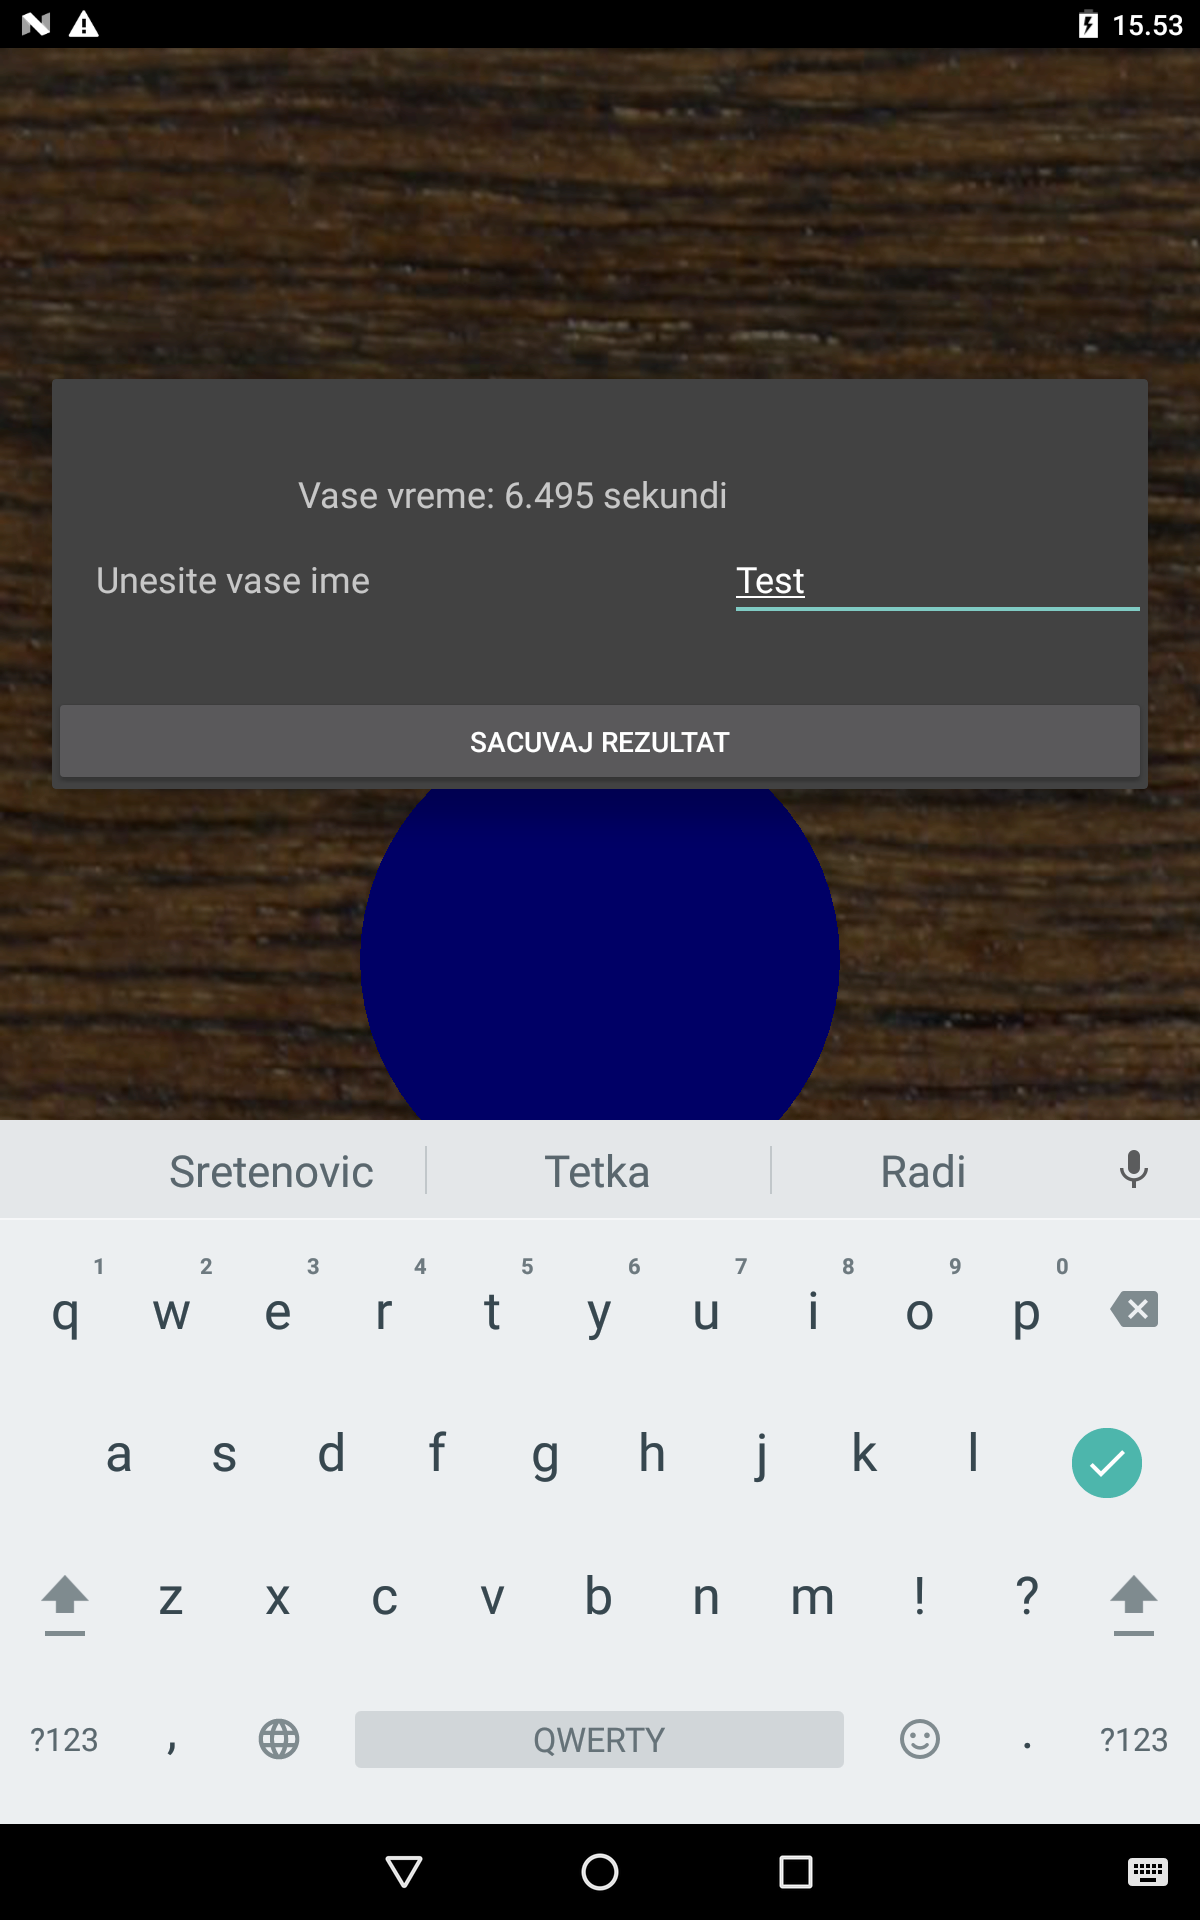
\includegraphics[scale=.1]{pictures/game/gameWon}
\caption{Дијалог кад победи}\label{fig:gameGameWon}
\end{center}
\end{figure}


\begin{figure}[htb!]
\begin{center}
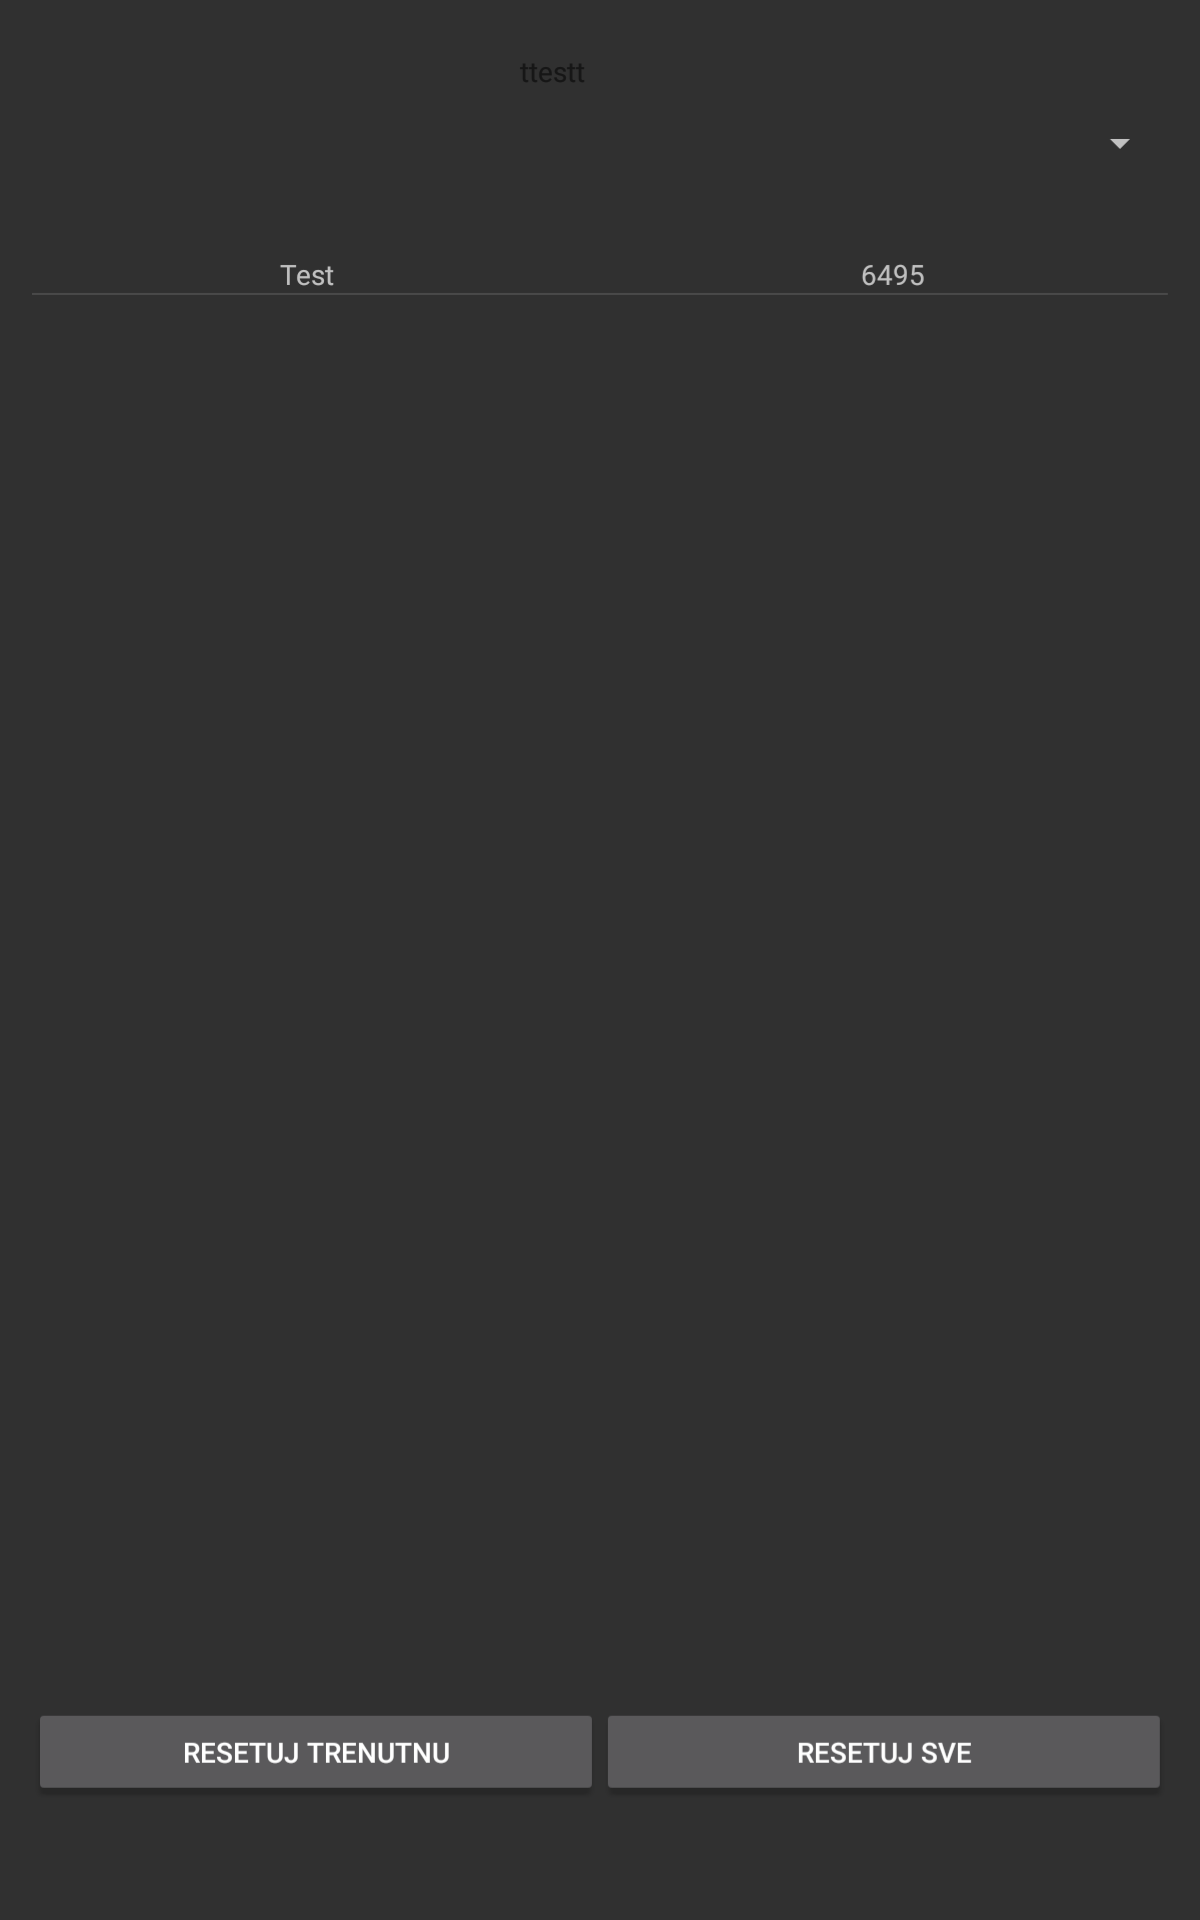
\includegraphics[scale=.1]{pictures/game/gameHighScore}
\caption{Листа резултата за полигон који је победио}\label{fig:gameGameHighScore}
\end{center}
\end{figure}

Кад корисник убаци лопту у зелену рупу, искаче му дијалог (слика \ref{fig:gameGameWon}). На дијалогу пише време, као и нуди кориснику да унесе своје име. Кад кликне на дугме \emph{SACUVAJ REZULTAT} корисников резултат се чува у листи резултата за тај плигон и отвара листа резултата за исти(слика \ref{fig:gameGameHighScore}).
\begin{figure}[htb!]
\begin{center}
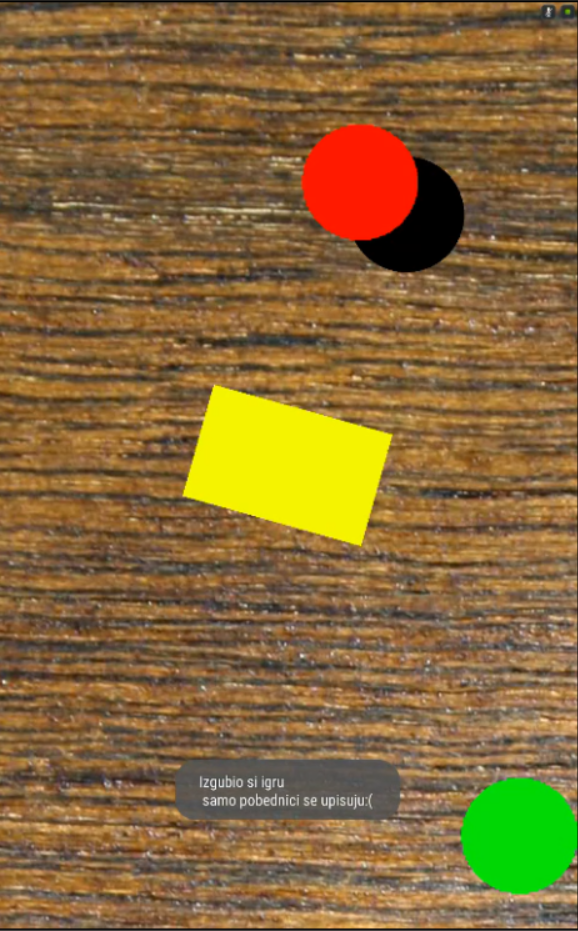
\includegraphics[scale=.4]{pictures/game/gameLose}
\caption{Обавештење кад корисник изгуби}\label{fig:gameLose}
\end{center}
\end{figure}
Када корисник упадне у амбис изађе му обавештење да је изгубио игру (слика \ref{fig:gameLose}). 

\section{Прављење полигона}\label{UseCases:CreatePolygon}
Постоје два мода у која корисник може да уђе кад уређује полигон. 
\\ \indent Један је мод уређивања, у ком се налази тако што или је кликнуо \emph{Uredi poligon} на почетном екрану или је сачувао полигон под неким именом. У овом моду кад корисник кликне назад аутоматски ће се чувати поруке и бити избацивана упозорења ако нешто није како треба (фали крајња позиција, почетна...). 
\\ \indent Други мод је обични мод и то је док корисник није сачувао полигон. У овом моду кад се кликне дугме назад, ништа неће бити сачувано. 
\begin{figure}[htb!]
\begin{center}
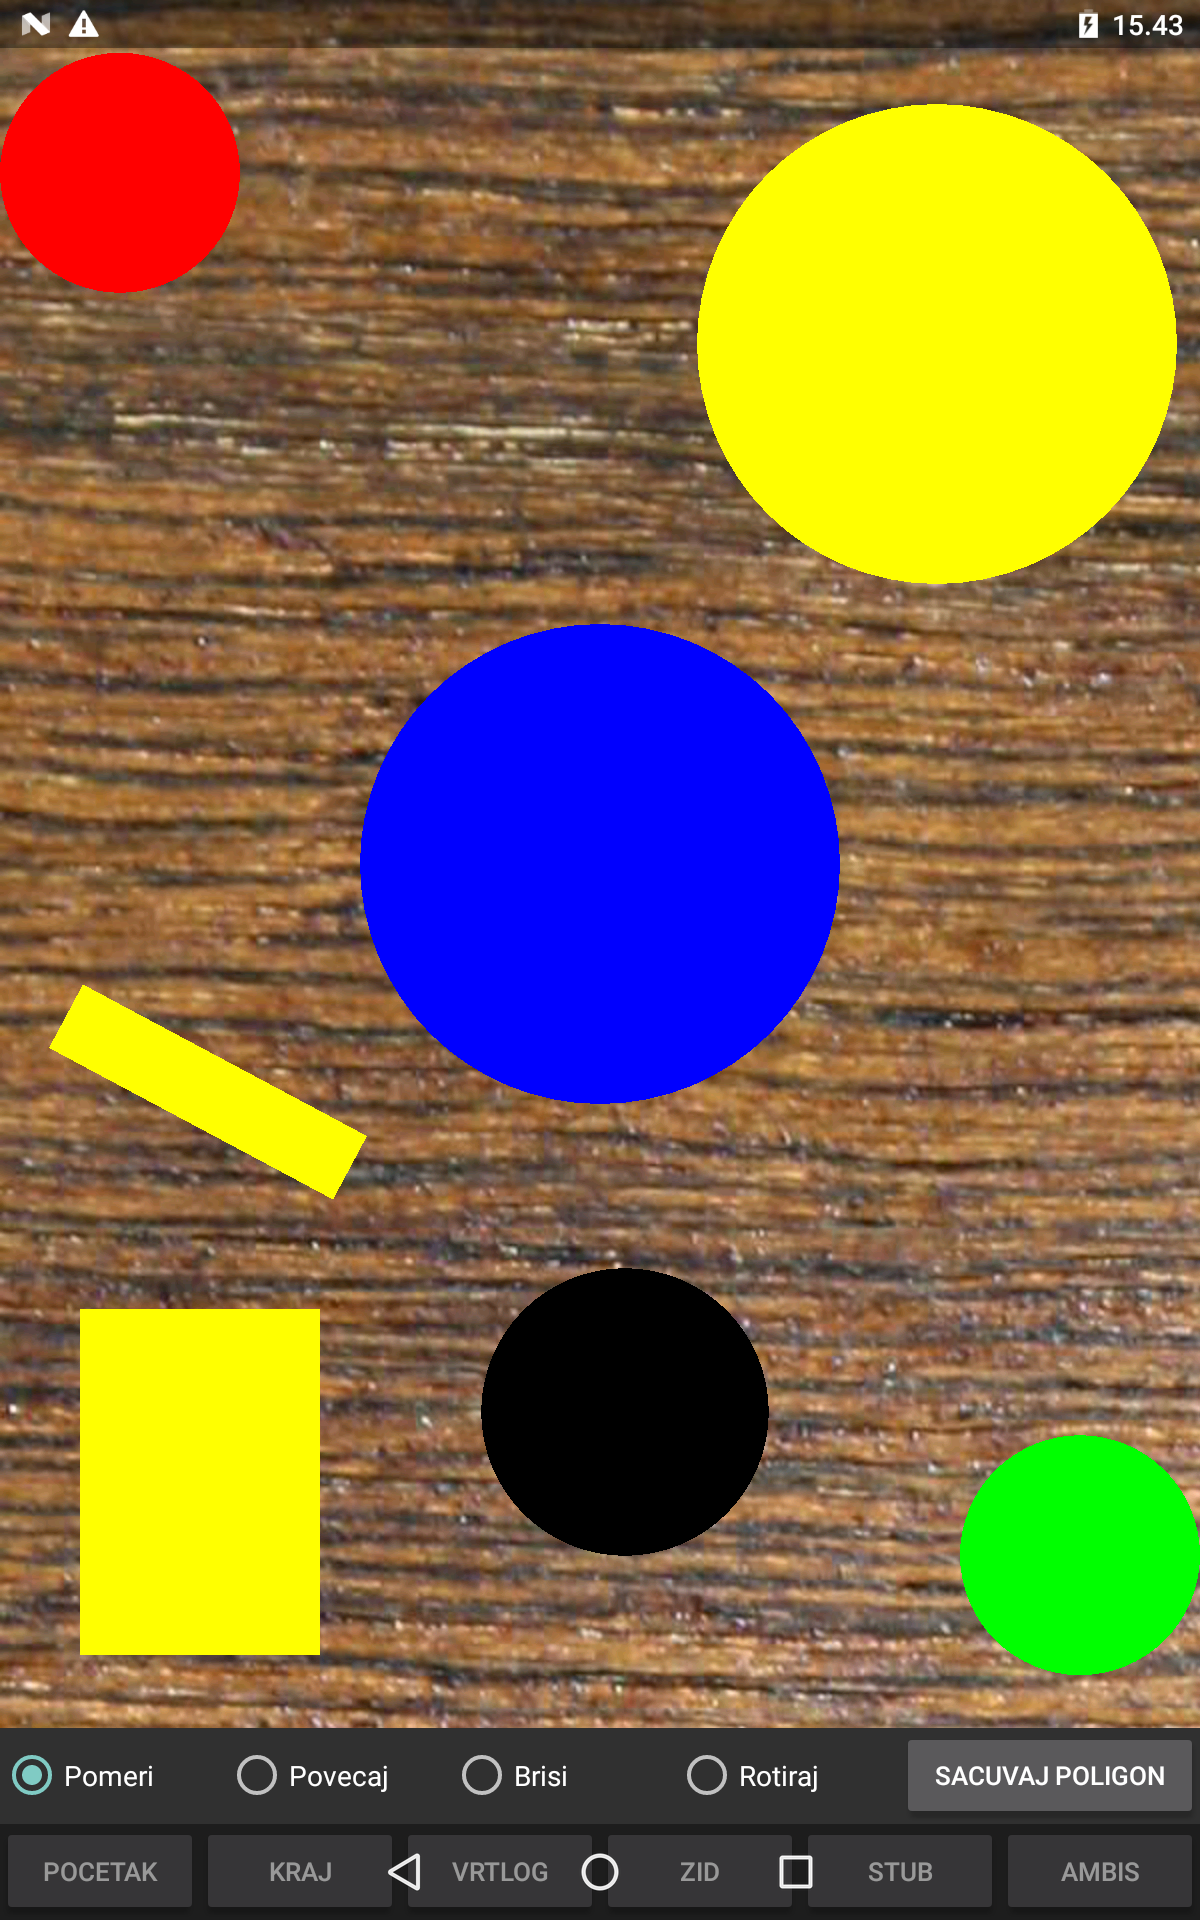
\includegraphics[scale=.1]{pictures/createPolygon/Basic}
\caption{Екран који корисник види кад уређује полигон}\label{fig:createPolygonBasic}
\end{center}
\end{figure}
Корисник има опције генерисања препрека за лопту наведеним у секцији \ref{UseCases:Game} кликтањем одговарајућег дугмета са именом. Такође може и да генерише почетну позицију лопте.  Поред тога са свим фигурама корисник може да ради једну од четири опције:
\begin{enumerate}
\item  \emph{Pomeri} - Помера одговарајућу фигуру на полигону тако да корисник мора да задржава прст на фигуи док је помера, Кад пусти, ту ће фигура бити померена. 
\item  \emph{Povecaj}- Повећава одговарајућу фигуру, тако да ако корисник одабере фигуру и помера прст, фигура ће се повећавати у односу на то где је његов прст (за круг ће крајња позиција прста означавати позицију тачке са кружнице, за правоугаоник позицију одговарајућег темена).
\item  \emph{Brisi} - Брише  одабрану фигуру са полигона.
\item  \emph{Rotiraj} - Ротира правоугаоник према позицији прста тако да одабрана права која је одређена центром правоугаоника и прстом ротира око центра пратећи прст, са том правом ротира и цео правоугаоник. 
\end{enumerate}

\begin{figure}[htb!]
\begin{center}
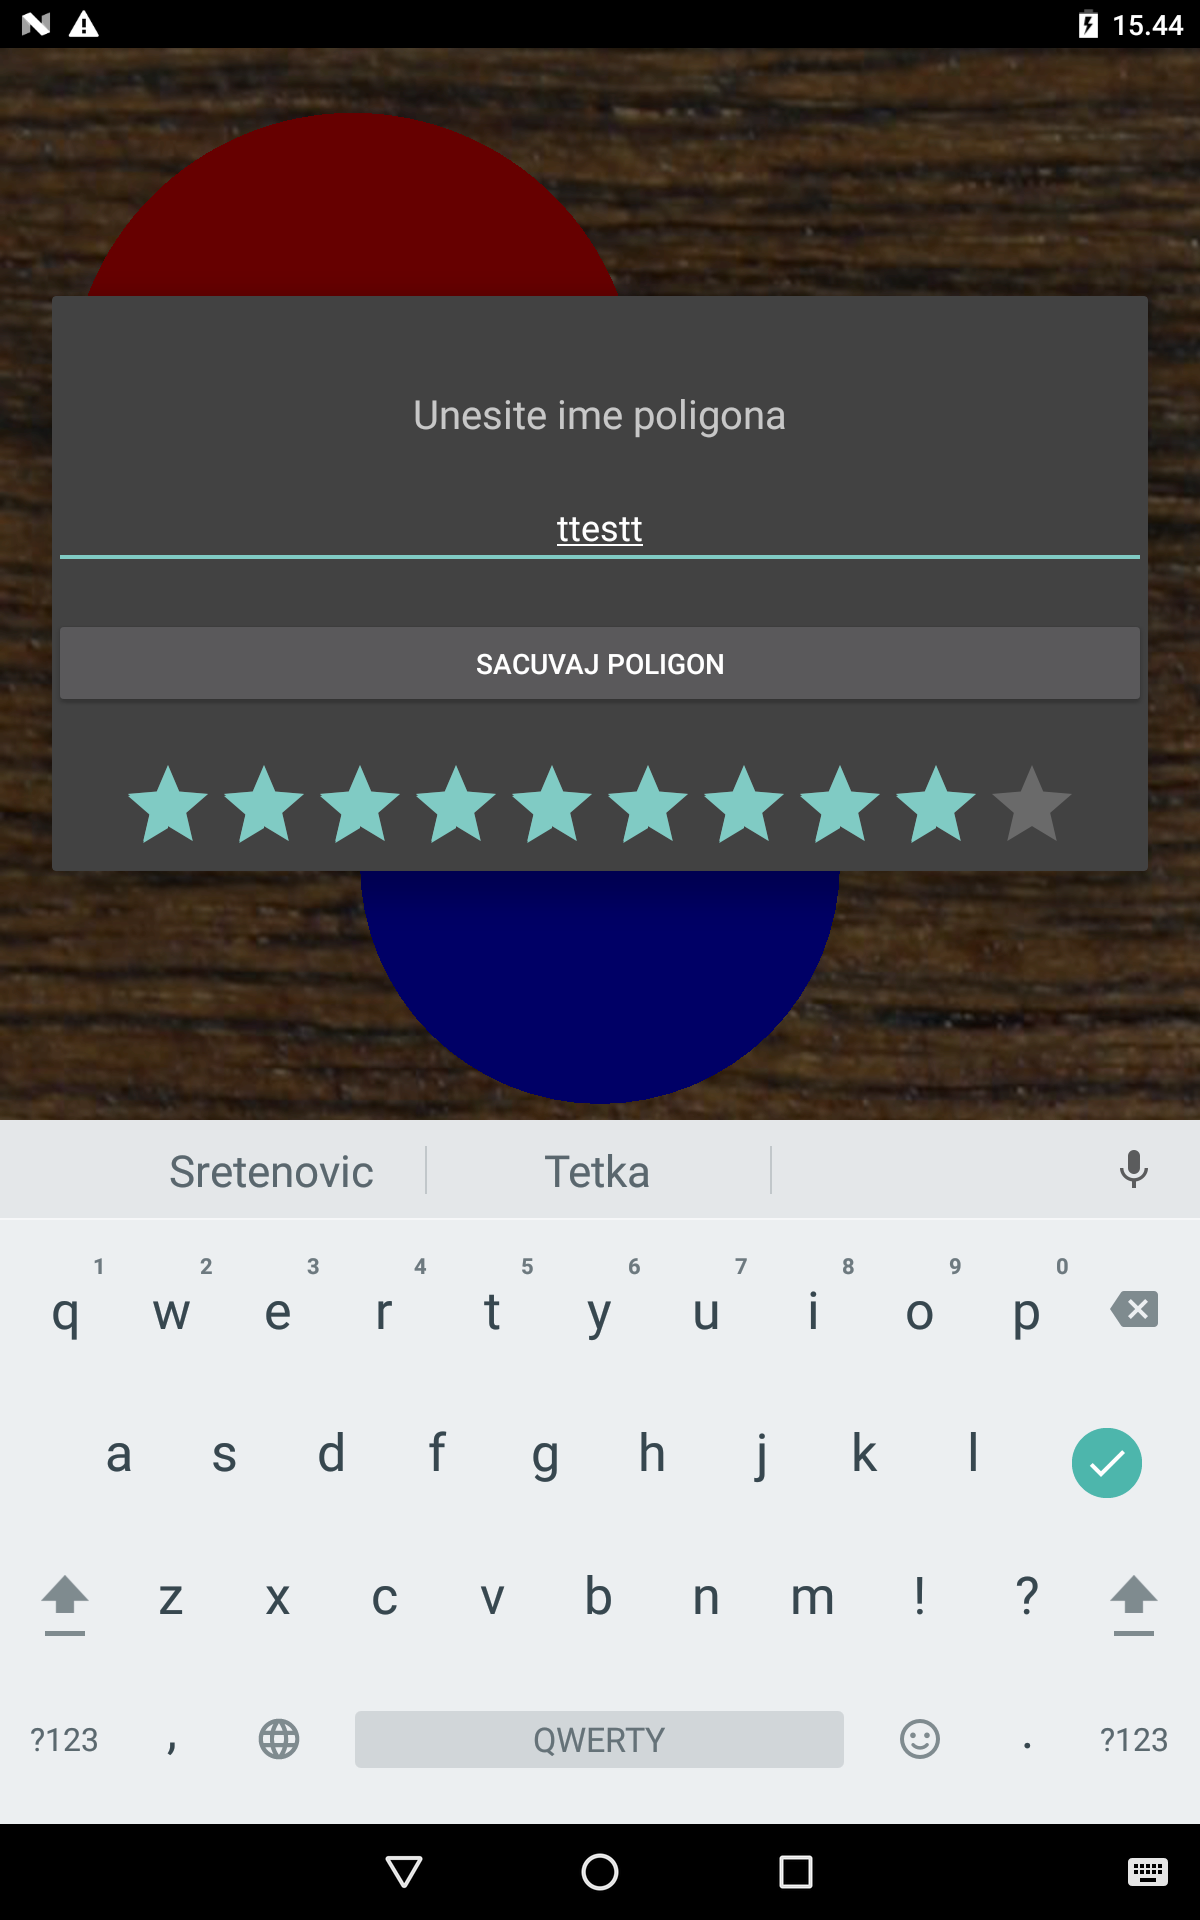
\includegraphics[scale=.1]{pictures/createPolygon/Save}
\caption{Дијалог који се појави кад корисник хоће да сачува полигон}\label{fig:createPolygonSave}
\end{center}
\end{figure}
На крају корисник кад заврши генерисање правоугаоника има дугме \emph{SACUVAJ POLIGON}. Тад се кориснику појављује дијалог на коме уноси тежину полигона као и име тог полигона. Кад кликне \emph{SACUVAJ POLIGON} на новом дијалогу, сачуваће полигон. Ако је постојао стари пребрисаће га.


\section{Резултати}\label{UseCases:Statistics}
\begin{figure}[htb!]
\begin{center}
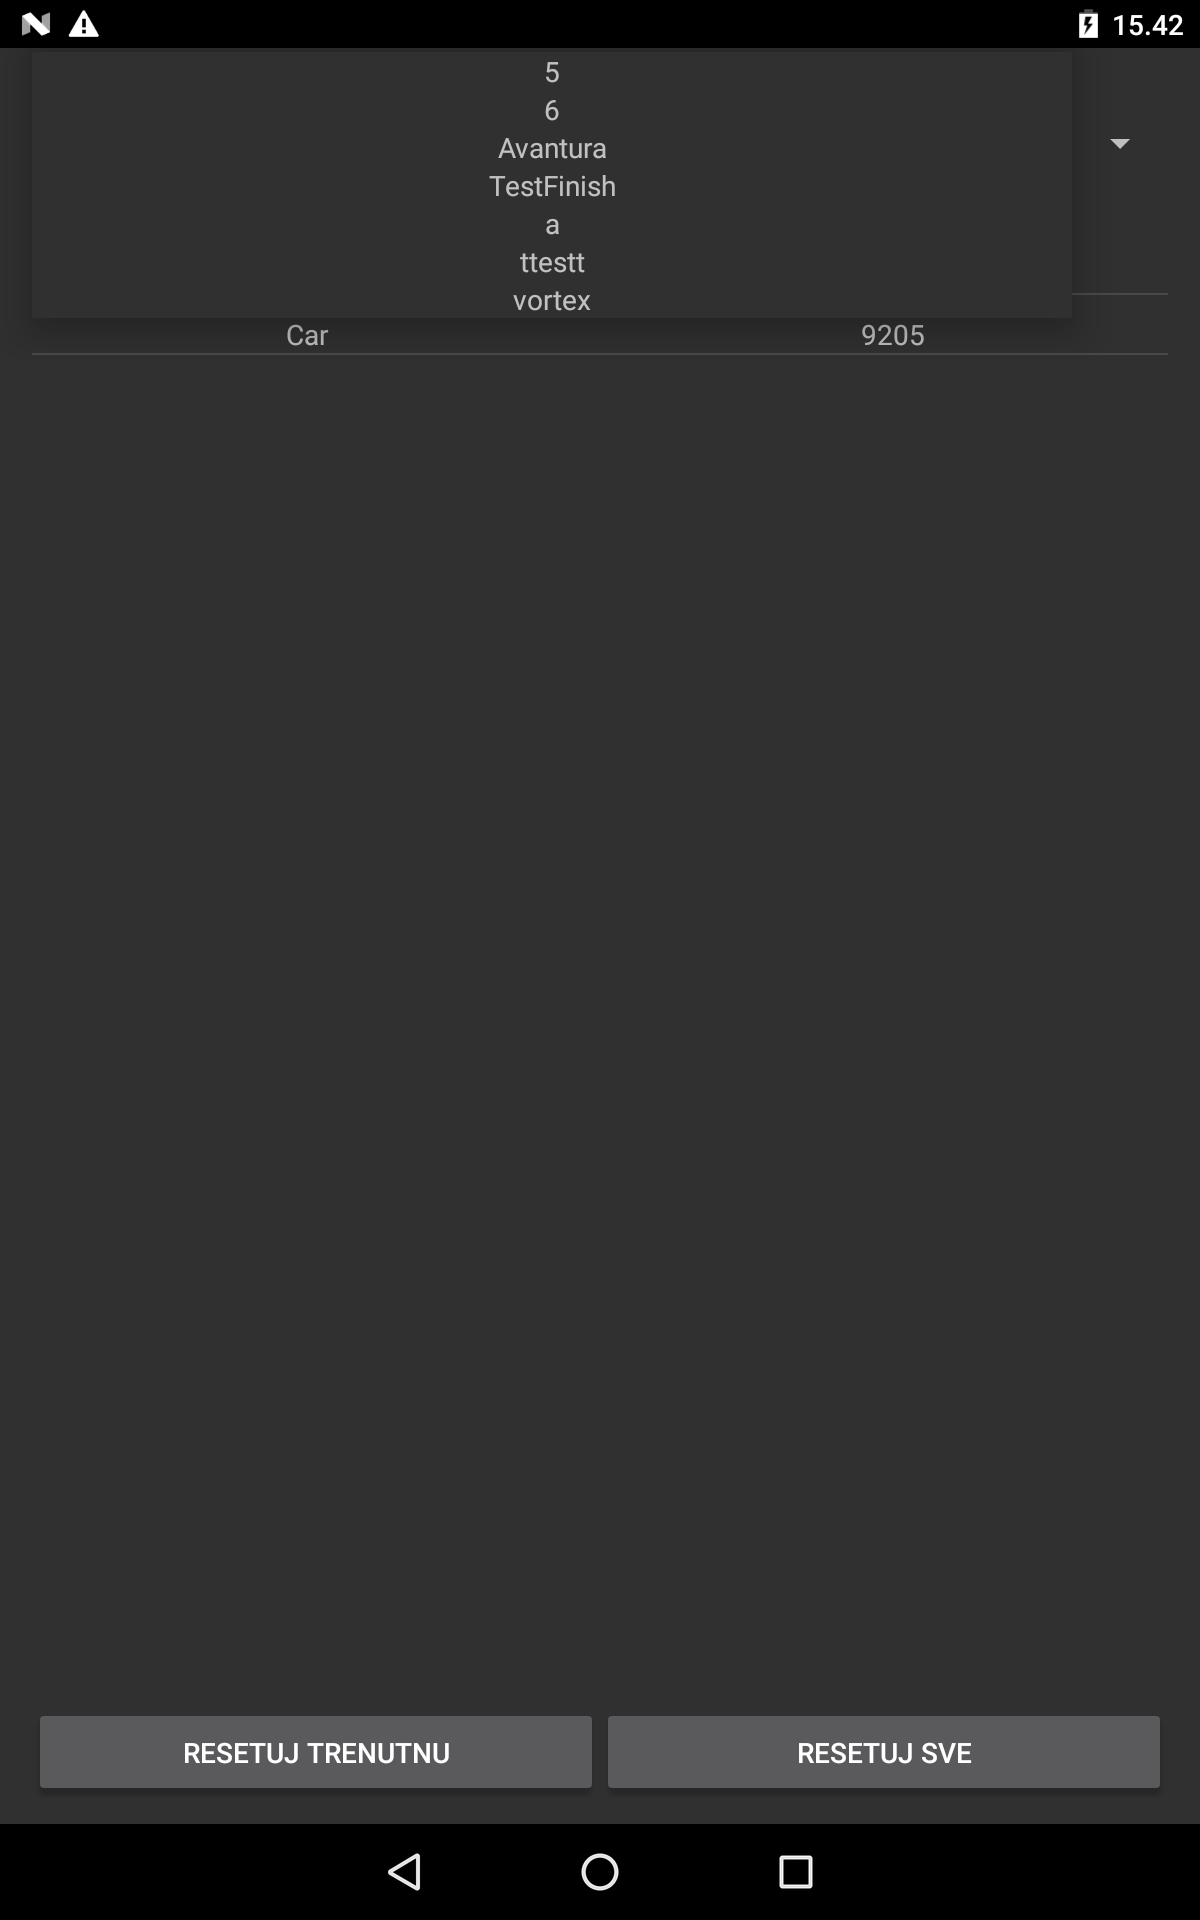
\includegraphics[scale=.1]{pictures/statistics/Choose}
\caption{Избор полигона за који хоће да се виде резултати}\label{fig:statisticChoose}
\end{center}
\end{figure}

\begin{figure}[htb!]
\begin{center}
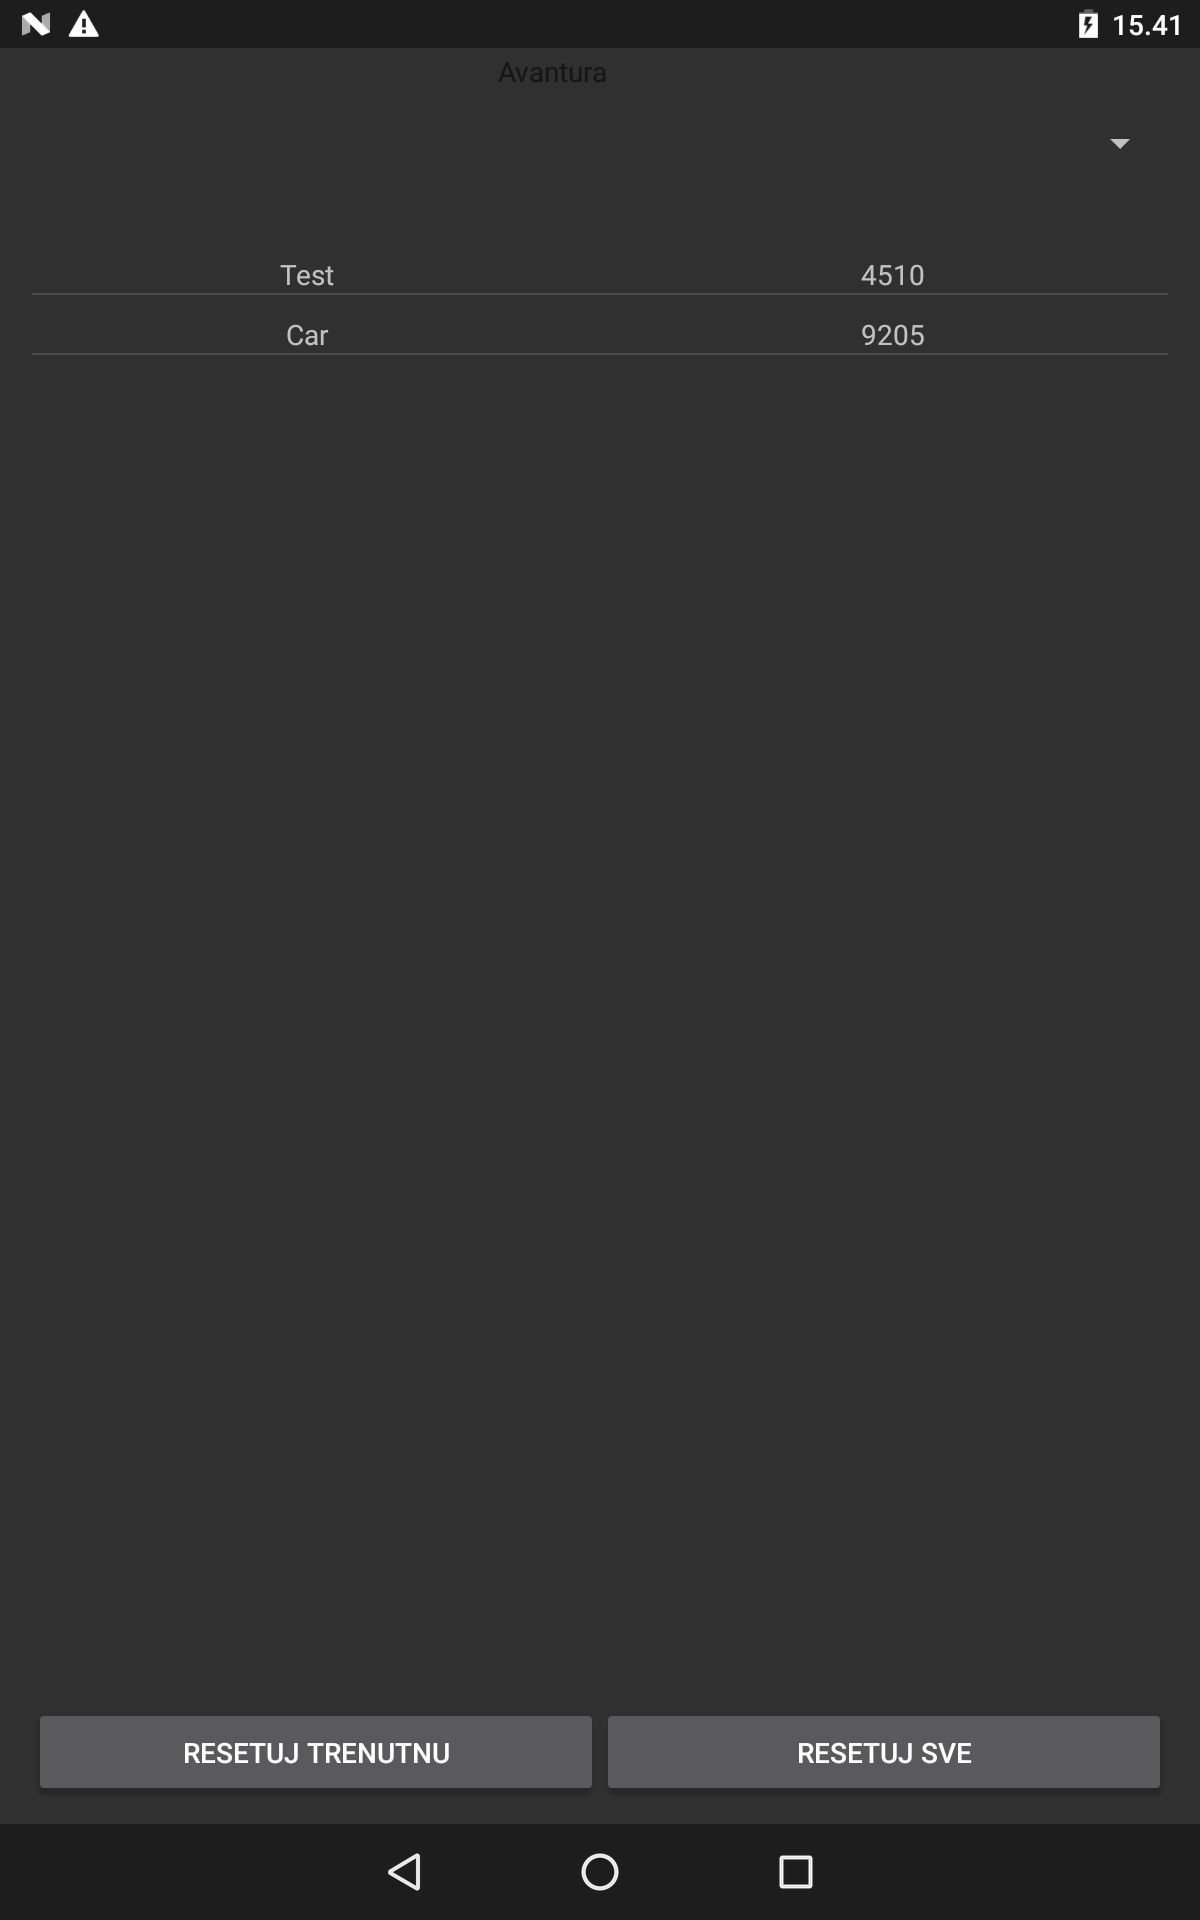
\includegraphics[scale=.1]{pictures/statistics/HighScore}
\caption{Листа резултата за одговарајући полигон}\label{fig:statisticHighScore}
\end{center}
\end{figure}
Корисник има опцију да види статистику за све полигоне које је играо, и који постоје . Такође има моућност да види и за авантура мод (под именом \emph{Avantura}). Корисник кликом на спинер бира одговарајући ниво за који хоће да прикаже резултате (слика \ref{fig:statisticChoose}) и потом, му се приказују резултати сортирани од најбољег ка најлошијем (\ref{fig:statisticHighScore}) у погледу времена. Корисник има могућност ресетовања листе резултата за један изабрани полигон притискањем дугмета \emph{RESETUJ TRENUTNU} или ресетовањем резултата свих листи са притискањем дугмета \emph{RESETUJ SVE}.


\section{Подешавања}\label{UseCases:Settings}
\begin{figure}[htb!]
\begin{center}
\includegraphics[scale=.1]{pictures/settings/basic}
\caption{Подешавања за игру}\label{fig:settingsBasic}
\end{center}
\end{figure}
Корисник има опцију да подеси одговарајуће коефицијенте  које се користе током симулације игре (слика \ref{fig:settingsBasic}). То се постиже померањем одговарајуће тачке на дужи. Редом су наведени коефицијенти:
\begin{enumerate}
\item Коефицијент убрзања - Колико брзо ће лоптица да убрзава, што већи коефицијент брже убрзава.
\item Коефицијент губитка брзине - Колико енергије остаје у лоптици приликом судара, што већи коефицијент, више енергије остаје.
\item Коефицијент трења - Колико лоптица успорава приликом кретања по подози, што већи коефицијент више успорава.
\end{enumerate}
Корисник има могућност да врати подешавања свих коефицијената на подразумевана притиском на дугме \emph{RESET} из одговарајућег реда за коефицијенте. 




\chapter{Android}\label{Android}

\emph{Још од избацивања IPhone-а као првог комерцијалног "паметног" телефона који ће објединити у једном уређају све функционалности  које има PC (линк \cite{IPHONE}), ако не и више, било је јасно у ком смеру се запутило IT \footnote{ Internet Technology} тржиште. Телефони или ти компјутери у џепу су у том тренутку постали будућност, а наша садашњост. Како ће се развијати IT технологија, није познато, али зна се да ће огроман удео имати телефони. Одатле и потиче моја  жеља да овладам вештином Android програмирања, оперативним системом који је преузео примат на тржишут паметних телефона. (линк \cite{MarkShare}) }
\section{GUI код}
Сав GUI који је коришћен, писан је у xml-у који подржва одговарајуће Android Studio IDE. Сва имена GUI компоненти давана су тако да прво иде тип компоненте и затим се надовезује одговарајући опис који је карактеристичан за употребу дате компоненте. Типа \emph{seekBarCoeficientAcceleration} означава \emph{seekBar} GUI компоненту, а CoeficientAcceleration каже да се користи да представи коефицијент убрзања. Имена сва су писана CamelCase-ом \footnote{\url{http://wiki.c2.com/?CamelCase}}. При избору компоненти биране су тако да што пријатније изгледа кориснику и да што лагодније буде за рад (на основу узорка од неколико корисника који су пробали различите верзије GUI-а). 
\\ \indent 
Где је било неопходно да позиционирање компоненти буде независно од типа од екрана коришћен је \emph{LinearLayout}
\footnote{\url{https://developer.android.com/reference/android/widget/LinearLayout.html}}, 
док је за неке ствари где је битна само позиција компоненти, коришћен \emph{RelativeLayout}\footnote{\url{https://developer.android.com/guide/topics/ui/layout/relative.html}}.
\\ \indent 
Коришћена је Android Dark Material Theme као основна тема.

\section{Java код}
GUI компоненте на одговарајућим екранима референциране су тако што се из одговарајућег прозора нађе компонента уз помоћ \emph{findViewById} \footnote{\url{https://developer.android.com/reference/android/view/View.html} и \url{https://developer.android.com/reference/android/app/Activity.html}}
\\ \indent 
Постоји пет активности (\emph{MainActivity, CreatePolygonActivity, GameActivity, SettingsActivity, StatisticsActivity}). Свака подржавајући одговарајућу функционалност из главе \ref{UseCases}. Дакле MainActivity почетни екран (\ref{UseCases:Main}), GameActivity  саму игру (\ref{UseCases:Game}), SettingsActivity подешавања (\ref{UseCases:Settings}), StatisticsActivity резултате (\ref{UseCases:Statistics}) и CreatePolygonActivity уређивање полигона (\ref{UseCases:CreatePolygon}).
\\ \indent 
Свака активност је прављена тако да је изведена из активности \emph{CommonActivtity}. Свака активност која наслеђује ову класу има подешен прозор тако да је навигациона трака скривена док корисник не превуче прстом са дна уређаја на горе. Поред тога оријентација је увек вертикално, да корисник не би губио време ако случајно окрене уређај. Такoђе екран обавештења је остао доступан кориснику да би могао у сваком тренутку да сазна више о обавештењу које му стигне (али тек након што превуче прстом екран са врха ка дну).
 Дата имплементације је по узору на већину данашањих екслузивних играчких наслова за Android уређаје попут Hill Climb Racing (линк за преузимање \cite{HillCR}). Даље коришћен је MVC\footnote{Model View Controller} пројектни узорак прилагођен за Android. При чему имамо активност која прослеђује своје догађаје контролеру, и он у зависности од њих обавља акције и у моделу се то чува. Постоји и имплементација где у моделу постоје методе које обрађују податке, али изабраним је раздвојена имплементација кода , од приступа подацима, и олакшана читкоћа кода.  Тамо где није био велики обим потребних метода (MainActivity, StatisticsActivity и SettingsActivity) обједињени су Controller и View. 
 \\ \indent
 Постојање класе \emph{CommonModel} за циљ има омогућавање заједничког модела свим активностима које су за потребу имали рендеровање направљеног/који се прави полигона. 
 \\ \indent
 Тамо где је разумно било да се појављују дијалози (као за чување резултата по успешној игри, или за чување направљеног полигона) прављене су класе (\emph{SaveDialog} и \emph{GameOverDialog}) које проширују класу 
 \emph{Dialog}\footnote{\url{https://developer.android.com/reference/android/app/Dialog.html}} и праве одговарајући потребан GUI. 
 Ово је омогућило финије подешавање дијалога и њиховог изгледа oд унапред направљених класа попут \emph{AlertDialog}\footnote{\url{https://developer.android.com/reference/android/app/AlertDialog.html}}.
\\ \indent 
Тамо где су била потребна исцртавања на екрану (\emph{CreatePolygonActivity} и \emph{GameActivity}) коришћене су одговарајућe класе које су проширивале \emph{SurfaceView} \footnote{\url{https://developer.android.com/reference/android/view/SurfaceView.html}} (биће касније објашњено како ово ради у глави \ref{Graphics}). 
\\ \indent 
За \emph{SettingsActivity} било је потребно  унапредити постојећу GUI компоненту SeekBar. Због тога је додата класа \emph{SeekBarUpgrade} која додаје још неки низ особина и омогућава лакше додавање више SeekBar-ова у SettingsActivity. 
\\ \indent 
Пошто је било неопходно да лопта реагује на силу која делује на Android уређај у \emph{GameActivity} активности , коришћен је уграђени Android сензор 
\emph{TYPE\_ACCELEROMETER}\footnote{\url{https://developer.android.com/guide/topics/sensors/sensors_overview.html}}.
Он сваких \si{20ms} прослеђује активности  детектоване вредности убрзања уређаја по \emph{x}, \emph{y} и \emph{z} оси. Њихово коришћење је описано даље у глави \ref{Collision}. Oва вредност од \si{20ms} емпиријским утврђивањем се показала као довољна да корисник стекне осећај реалистичности кретања куглице и реаговања исте на силе које делују на уређај. 
\\ \indent 
Да би корисник стекао што реалистичнији осећај кретања лоптице и тренутка њеног судара са препрекама или уласка у њих неопходно је било подржати звук. Изабрана је класа \emph{SoundPool}\footnote{\url{https://developer.android.com/reference/android/media/SoundPool.html}} која омогућава пуштање звукова. Имплемнтиран је омотач за њу у виду класе \emph{SoundPlayer} који додаје још неке функционалности. Звучни ефекти су одабрани емпиријски да што краће трају и да корисник не обража превелику пажњу на њих. Детаљније у методама, интерфејсу и свим класама за звукове у глави \ref{Architecture}.

\section{Чување података}
Постојале су потребе за три начина чувања података у апликацији. 
\\ \indent 
Први потребан начин је било перзистирање коефицијената потребних за симулацију кретања лопте. Пошто су они били потребн да перзистирају дуж активности \emph{GameActivity} и \emph{SettingsActivity} и није их било пуно, одбачене су опције да се чувају у бази и посебном фајлу. Стога је одабрана опција \emph{SharedPreferences}\footnote{\url{https://developer.android.com/reference/android/content/SharedPreferences.html}} која чува податке у облику пара key/value. Ово омогућава згодно додавање нове константе без гломазних мењања база и без мењања шеме фајла. Овај систем је имплементиран у класи \emph{Coefficient}.
\\ \indent 
Други потребан начин било је перзистирање података везаних за име нивоа, тежину, као и рангирање нивоа. То је омогућено коришћењем SQLite језика који је ништа друго него лакша варијанта SQL\footnote{Standard Query Language} језика за рад са базом. Прво је имплементиран \emph{SQLiteOpenHelper} у виду класе \emph{GameDatabaseHelper} који омогућава мењање шеме базе (ако се врши додавање нове функционалности у игрици везане за нивое), као и приступ истој. Даље је \emph{GameDatabaseHelper} омотан у класи \emph{GameDatabase} која имплементира читав низ функционалности који је био неопходан у апликацији. 
\\ \indent 
Последњи потребан начин било је перзистирање нивоа (њиховог изгледа). Одабран је начин чувања у фајловима. То омогућава згодно додавање нових фигура само додавањем новог типа фигуре, и не изискује гломазно мењање базе података и API-а функционалности базе. Пошто је било неопходно да се омогући перзистирање димензија фигура на полигону за сваки тип уређаја, то је урађено скалирањем фигура у односу на величину екрана. Скалирање фигура се обавља уз помоћ класa \emph{UtilScale} и \emph{UtilScaleNormal} (апстрактна и имплементација). Класа која чува полигоне у облику фајлова у овом формату је \emph{ShapeParser}. 

\section{Unit Test}
За потребе тестирања коришћени су корисници који су играли ову игрицу, као и \emph{JUnit} пакет који је омогућио тестирање одређених метода класа и функционалности. Да би ова апликација ишла у продукцију, неопходна су бројна унапређења у тестирању као и броју тестова.
\chapter{Модел судара} \label{Collision}

У овом поглављу биће изложен рад са класом 

\chapter{Графика} \label{Graphics}

\emph{Иако рачунарска графика на први поглед изгледа једноставна област, што се више задубљујеш у њу, откриваш каква озбиљна наука стоји. }

\section{Општа идеја}
Док су за активности у којима није потребно учестало исцртавања екрана коришћена GUI нит, тамо где је потребно (\emph{CreatePolygonActivity, GameActivity}) морало је бити пронађено другачије решење. За површ уместо стандардног \emph{Canvas}-a који припада \emph{ImageView}, који захтева исцртавање целог екрана \footnote{\url{https://developer.android.com/reference/android/widget/ImageView.html}} користи се \emph{SurfaceView} који се само освежи (остатак екрана се не мења) кад је неопходно. И то исцртавање се ради у посебној нити, која кад заврши посао, само замени \emph{Canvas} од SurfaceView са новим Canvas-ом. Што умањује заузетост GUI нити непотребним исцртавањем, и омогућава да се користи у рачунању и ажурирању SurfaceView.
Ради смањења загревања уређаја, нова нит која исцртава \emph{Canvas} то ради само кад је затражено од ње (кад се десила промена позиције), остатак времена спава. 
\\ \indent
 Цео модел је оптимизован тако да се тражило максималној паралелизацији и минимализацији броја lock-ова. У обе активности се на почетку иницијализације \emph{SurfaceView} правe класе \emph{ShapeFactory} и \emph{ShapeDraw}, од којих прва служи за парсирање полигона из фајлова (и њихово скалирање), док друга служи за цртање фигура по \emph{Canvas}-у \emph{SurfaceView}. Да би фигура била исцртана помоћу класе \emph{ShapeDraw} неопходno je да подржава \emph{ShapeDrawInterface}, тј. да може да се кликне на њу, ротира, промени величина, помери, израчуна угао нагиба. Такође при иницијализацији \emph{SurfaceView} прави се и посебна нит која ће да ради исцртавање. При уништавању \emph{SurfaceView} нит се уништава.
\section{Оптимизације код играња игре}
 Код играња игре, нема потребе за непотребно рендеровање и исцртавање других фигура по \emph{Canvas}-у осим на почетку. Стога се направи спрајт целог полигона без лопте, и лопта се лепи касније на спрајт како се мења њена позиција. Ово омогућава убрзано ажурирање екрана.
\chapter{Aрхитектура} \label{Architecture}

\section{Организација пакета}

\begin{figure}[htb!]
\begin{center}
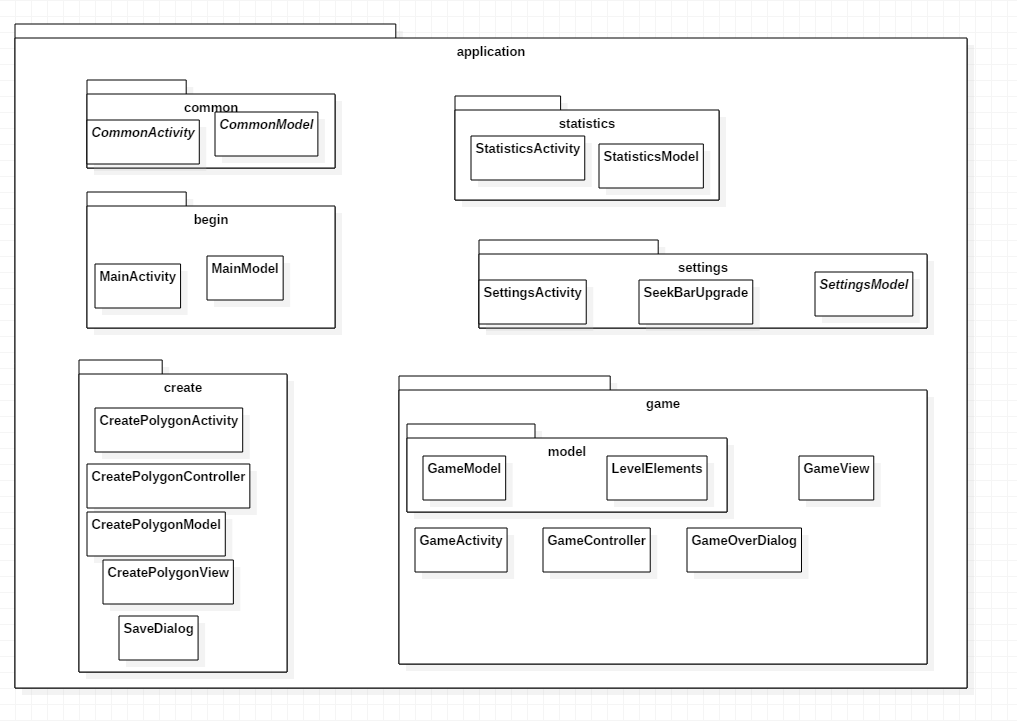
\includegraphics[scale=.7]{pictures/UML/package/application}
\caption{Организација класа по пакетима (application пакет)}\label{fig:umlPackageApp}
\end{center}
\end{figure}

\begin{figure}[htb!]
\begin{center}
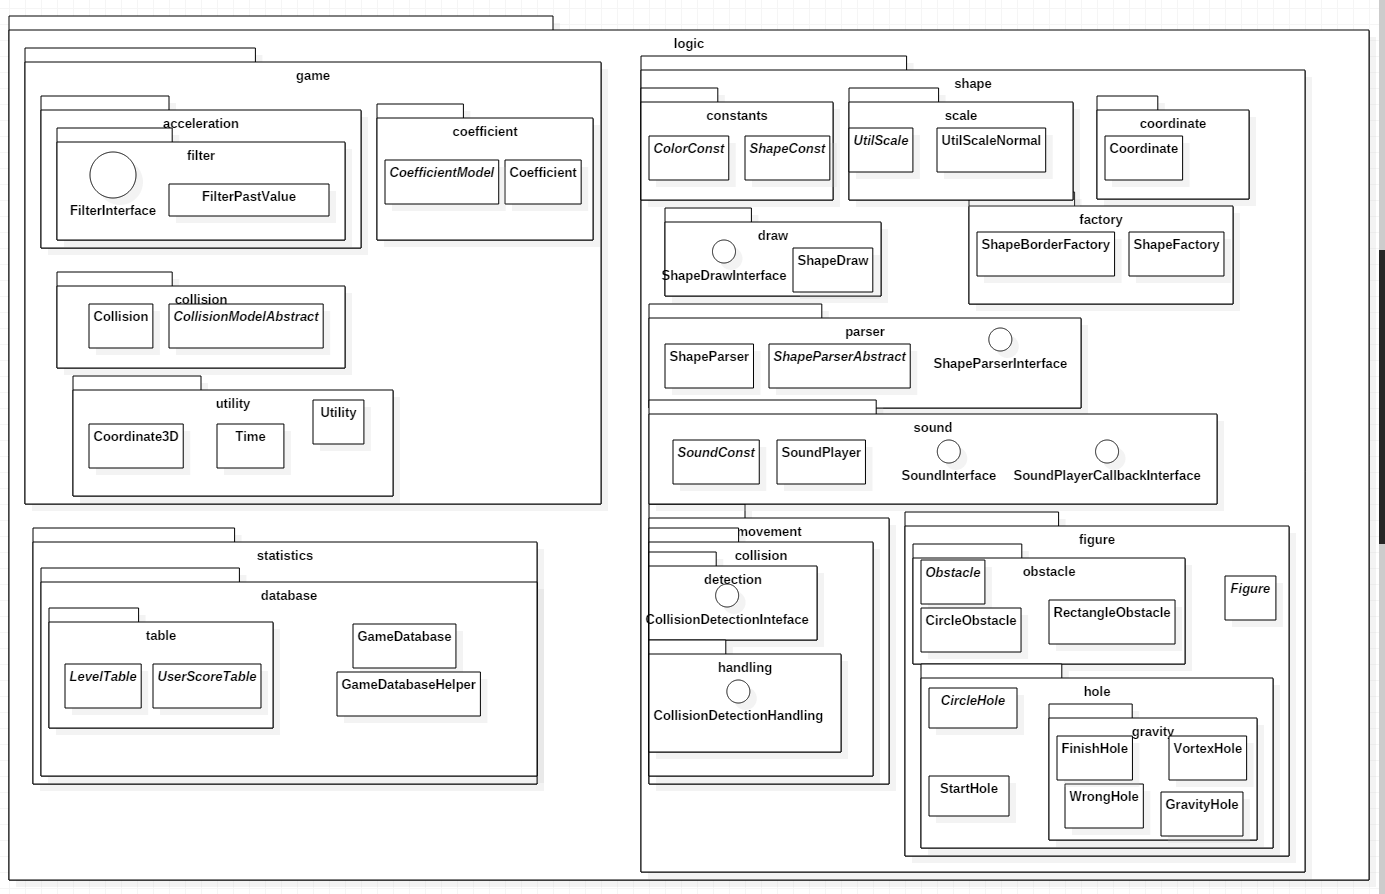
\includegraphics[scale=.6]{pictures/UML/package/logic}
\caption{Организација класа по пакетима (logic пакет)}\label{fig:umlPackageLog}
\end{center}
\end{figure}

Читав java код је организован тако да се налази унутар пакета \emph{com.example.popina.projekat} и то у два потпакета. Код који је везан за MVC преглед и Android део налази се у applicatiоn потпакету (слика \ref{fig:umlPackageApp}). Код који је везан за логику игре (база података, како се праве фигуре, парсира...) налази се у потпакету logic (\ref{fig:umlPackageLog}).
\chapter{Закључак} \label{Conclusion}

Игрица је за циљ имала учење Android API-а и његову употребу ради оптимизације пројекта. Али проблеми попут рачунарске графике и моделирања физике пребацили су тежиште пројекта.  
\\ \indent Стога игрица је постигла првобитни циљ, а то је Android апликација чији код је читак, добро организован, лак за проширивање. Додавање нових препрека у игри је веома једноставно проширивањем постојећих класа или имплементирањем интерфејса.. Додавање нових опција у модел физике је веома једноставно мењањем једне методе. Механика играња тј. исцртавња фигура апликације је оптимизована до границе кад корисник не осећа да се ради о Android уређају. У суштини, читав апликација је добро организована и проширива у свим погледима. 
\\ \indent Међутим проблем савршене физике остаје отворено питање. Модел који је урађен, довољан је да корисник не примети несавршеност физике у неким деловима. Међутим, требало би да се среди даљим изучавањем моделирања физике у оваквим типовима апликација. 
\\ \indent Следеће отворено питање да ли користити OpenGL и да ли ће он дати још већа побољшања у погледу исцртавања фигура. И са тим питање, да ли треба да се поред лопте која се креће треба да дода неколико покретних препрека. Да ли би оне кориснику дале још више уживања? Све ово захтева темељно испитивање OpenGL API-а за Anrdoid и његово темељно тестирање на одговарајућим моделима физике који буду коришћени.
\\ \indent Треће отворено питање је изглед апликације. Иако је уложен огроман  труд да се постигне да апликација буде што привлачнија за кориснике, видно је да неки делови захтевају побољшање (попут боја препрека, лопте, могућност постављања позадине нивоа).  Стога, треба наћи добро GUI дизајнера за Android који би средио претходно наведене мањкавости. 
\\ \indent Последње отворено питање је сама логика апликације, тј. како се ради adventure мод игрице, и да ли треба дозволити кориснику да прави сам нивое за тај мод. Стога треба извршити истраживање код корисника да се види шта они очекују од овакве апликације по питању нивоа.
\\ \indent И последње питање, да ли апликација треба да иде у продукцију (на Google Play Store линк: \cite{GooglePlayStore}). Ако буде постојала жеља, неопходно је систем тестирања подићи на виши ниво, темељно тестирати све методе и све могуће случајеве коришћења. 

\addcontentsline{toc}{chapter}{\bibname}





\begin{thebibliography}{15}
	\bibitem{BluetoothTerminal}
		NMinion.
		\emph{Bluetooth Serial Terminal}.\\
		\url{https://www.microsoft.com/en-us/store/p/bluetooth-serial-terminal/9wzdncrdfst8}
		


\end{thebibliography}

\end{document}